\documentclass[11pt,]{article}
\usepackage{lmodern}
\usepackage{amssymb,amsmath}
\usepackage{ifxetex,ifluatex}
\usepackage{fixltx2e} % provides \textsubscript
\ifnum 0\ifxetex 1\fi\ifluatex 1\fi=0 % if pdftex
  \usepackage[T1]{fontenc}
  \usepackage[utf8]{inputenc}
\else % if luatex or xelatex
  \ifxetex
    \usepackage{mathspec}
    \usepackage{xltxtra,xunicode}
  \else
    \usepackage{fontspec}
  \fi
  \defaultfontfeatures{Mapping=tex-text,Scale=MatchLowercase}
  \newcommand{\euro}{€}
    \setmainfont{Georgia}
\fi
% use upquote if available, for straight quotes in verbatim environments
\IfFileExists{upquote.sty}{\usepackage{upquote}}{}
% use microtype if available
\IfFileExists{microtype.sty}{%
\usepackage{microtype}
\UseMicrotypeSet[protrusion]{basicmath} % disable protrusion for tt fonts
}{}
\usepackage[margin=1.0in]{geometry}
\ifxetex
  \usepackage[setpagesize=false, % page size defined by xetex
              unicode=false, % unicode breaks when used with xetex
              xetex]{hyperref}
\else
  \usepackage[unicode=true]{hyperref}
\fi
\hypersetup{breaklinks=true,
            bookmarks=true,
            pdfauthor={},
            pdftitle={},
            colorlinks=true,
            citecolor=blue,
            urlcolor=blue,
            linkcolor=magenta,
            pdfborder={0 0 0}}
\urlstyle{same}  % don't use monospace font for urls
\usepackage{graphicx,grffile}
\makeatletter
\def\maxwidth{\ifdim\Gin@nat@width>\linewidth\linewidth\else\Gin@nat@width\fi}
\def\maxheight{\ifdim\Gin@nat@height>\textheight\textheight\else\Gin@nat@height\fi}
\makeatother
% Scale images if necessary, so that they will not overflow the page
% margins by default, and it is still possible to overwrite the defaults
% using explicit options in \includegraphics[width, height, ...]{}
\setkeys{Gin}{width=\maxwidth,height=\maxheight,keepaspectratio}
\setlength{\parindent}{0pt}
\setlength{\parskip}{6pt plus 2pt minus 1pt}
\setlength{\emergencystretch}{3em}  % prevent overfull lines
\providecommand{\tightlist}{%
  \setlength{\itemsep}{0pt}\setlength{\parskip}{0pt}}
\setcounter{secnumdepth}{0}

%%% Use protect on footnotes to avoid problems with footnotes in titles
\let\rmarkdownfootnote\footnote%
\def\footnote{\protect\rmarkdownfootnote}

%%% Change title format to be more compact
\usepackage{titling}

% Create subtitle command for use in maketitle
\newcommand{\subtitle}[1]{
  \posttitle{
    \begin{center}\large#1\end{center}
    }
}

\setlength{\droptitle}{-2em}
  \title{}
  \pretitle{\vspace{\droptitle}}
  \posttitle{}
  \author{}
  \preauthor{}\postauthor{}
  \date{}
  \predate{}\postdate{}

\usepackage{booktabs}
\usepackage{changes}
\usepackage[font={small},labelfont=bf,labelsep=colon]{caption}
\linespread{1.5}
\usepackage[compact]{titlesec}
\usepackage{enumitem}
\usepackage{tikz}
\def\checkmark{\tikz\fill[scale=0.4](0,.35) -- (.25,0) -- (1,.7) -- (.25,.15) -- cycle;}
\setlist{nolistsep}
\titlespacing{\section}{2pt}{*0}{*0}
\titlespacing{\subsection}{2pt}{*0}{*0}
\titlespacing{\subsubsection}{2pt}{*0}{*0}
\setlength{\parskip}{3pt}
\setremarkmarkup{(#2)}
\definechangesauthor[name={Nick Tustison}, color=red]{nt}
\definechangesauthor[name={James Stone}, color=magenta]{js}
\definechangesauthor[name={Lisa Wilde}, color=cyan]{lw}
\definechangesauthor[name={Andy Mayer}, color=green]{am}
\definechangesauthor[name={Harvey Levin}, color=blue]{hl}
\definechangesauthor[name={Brian Taylor}, color=purple]{bt}

% Redefines (sub)paragraphs to behave more like sections
\ifx\paragraph\undefined\else
\let\oldparagraph\paragraph
\renewcommand{\paragraph}[1]{\oldparagraph{#1}\mbox{}}
\fi
\ifx\subparagraph\undefined\else
\let\oldsubparagraph\subparagraph
\renewcommand{\subparagraph}[1]{\oldsubparagraph{#1}\mbox{}}
\fi

\begin{document}
\maketitle

\pagenumbering{gobble}

\section{Introduction}\label{introduction}

\subsection{White matter hyperintensities in
TBI}\label{white-matter-hyperintensities-in-tbi}

White matter hyperintensities (WMHs) are foci of abnormally increased
signal intensity seen within white matter regions within the cerebrum
and brainstem on fluid attenuation inversion recovery (FLAIR) magnetic
resonance imaging (MRI) sequences. These lesions are distinguished from
prominent perivascular spaces seen on T2-weighted imaging by the lack of
fluid suppression of signal on FLAIR sequences. WMHs in the
periventricular and deep brain regions are associated with normal aging
and neurological conditions including hypertension and stroke. WMHs are
also a frequent finding following traumatic brain injury (TBI) and have
been correlated with functional outcome and injury severity in both
pediatric {[}1, 2{]} and adult {[}3--6{]}. Further, the regional
distribution and volume of WMHs have been shown to possess prognostic
value in the TBI patient {[}2, 6--8{]}. Specifically, lesion volume in
corpus callosum correlates with functional scores in the acute phase
following injury, while lesion volume in frontal lobes correlates with
scores at 1 year following injury {[}6{]}. Further, volume of FLAIR
lesions within the corpus callosum, brainstem, and thalamus in patients
with severe TBI correlates with Glasgow Outcome-Extended (GOS-E) scores
{[}4{]}. Additionally, the regional distribution of FLAIR lesions within
the pons, midbrain, hypothalamus, basal forebrain, parietal, temporal,
occipital lobes, and insula along with the observation of grasping or
chewing behavior are associated with poor outcome {[}7{]}.

Despite the above findings, outside of multiple sclerosis, WMHs are not
routinely employed as a diagnostic measure in clinical practice. Their
presence within asymptomatic patients or in association with a variety
of conditions, such as stroke, dementia, neuroinflammatory conditions,
and TBI challenge their utility in narrowing a radiological differential
diagnosis. Further, performing a comprehensive manual counting of number
and distribution of lesions in the clinical setting is simply not
practical. Despite the limited inclusion of WMH observations in routine
radiological reports, two large meta-analyses demonstrated an
association between WMHs, cognitive function, increased risk of stroke,
dementia, and death {[}9, 10{]}. As such, the development of automated
methods for the rapid identification and quantification of WMHs within
individual patients may allow for identification of correlative patterns
between WMH number, volume, distribution, and disease state. Further,
the development of such lesion quantification approaches may allow for
the practical inclusion of this type of information within routine
radiological practice.

\subsection{Random forests for WMH
segmentation}\label{random-forests-for-wmh-segmentation}

Machine learning and pattern recognition techniques have seen increased
application for various medical image analysis workflows (see, for
example, the annual Workshop on Machine Learning in Medical Imaging held
in conjunction with the Medical Image Computing and Computer-Aided
Intervention (MICCAI) international meeting {[}11{]}). Popular
techniques such as support vector machines and neural networks have been
applied successfully to clinically relevant imaging tasks such as
supervised image segmentation (e.g., {[}12{]}) and diagnostic prediction
(e.g., {[}13, 14{]}). Facilitating the current employment of such
techniques are the number of available imaging data sets {[}15{]} and
the public availability of data science packages such as SciPy {[}16{]}
and the R project for statistical computing {[}17{]} and their
associated extensions.

The random forests framework {[}18{]} is a popular machine learning
technique that has demonstrated significant utitility for supervised
segmentation tasks (e.g., normal human brain segmentation {[}19{]}) and
other computer vision applications (e.g., human gait detection
{[}20{]}). In the context of neuropathology, random forest-based
paradigms have been employed in the delineation of multiple sclerosis
lesions {[}21{]}, stroke lesions {[}22{]}, and brain tumors
{[}23--26{]}. Of note, these latter random forest approaches for brain
tumor segmentation have performed well in recent international
competitions. In response to the lack of objective comparisons between
segmentation algorithms, the Multimodal Brain Tumor Segmentation (BRATS)
challenge was initiated in 2012 {[}27{]} and has continued every year
since under the auspices of the MICCAI conference.

Random forests are conceptually simple {[}18{]}. They consist of
ensembles of decision trees that are built from training data. Once
constructed, data to be classified is ``pushed'' through each decision
tree resulting in a single classification ``vote'' per tree. These votes
are then used for regression or classification of the data. Although
decision trees had been extensively studied previously, the success of
employing collections of such weak learners for boosting machine
learning performance (e.g., AdaBoost {[}28, 29{]}) influenced the
similarly sytled conglomeration of decision trees into ``forests'' with
randomized node optimization {[}30, 31{]}. Finally, Breiman {[}18{]}
improved accuracy by random sampling of the training data (i.e.,
``bagging'') resulting in the current random forest technique.

In this work, we develop a concatenated random forest framework with a
tailored contextual feature image set (both spatial and intensity-based)
for segmenting white matter hyperintensities in traumatic brain injury
cohorts. Additionally, the entire framework is provided publicly through
the well-known open-source ANTs\footnote{\url{https://github.com/stnava/ANTs}}
and ANTsR\footnote{\url{https://github.com/stnava/ANTsR}} toolkits.
Further motivating the research of this work is the public availability
of the imaging data thus permitting full reproducibility of the results
reported and discussed.

\section{Materials and Methods}\label{materials-and-methods}

\subsection{Imaging}\label{imaging}

MR images utilized for this initial report were acquired from 24
individuals scanned at a single site involved in the Chronic Effects of
Neurotrauma Consortium's (CENC) observational study
(\added[id=nt,remark=NT: reference needed?]{see [Walker], this issue}).
Briefly, participants were Operation Enduring Freedom/ Operation Iraqi
Freedom /Operation New dawn (OEF/OIF/OND) era service members and
veterans between the ages of 18--60 who have experienced combat
situations and are between X and X (period of time) from deployment.
\added[id=js,remark={JS: Data needed.}]{The feature images consisted of subjects aged $X.X \pm X$ years (range X – X years), XX percent male, with at least one or more potential concussive events (mean = X, SD = X, range X-X).}

Images were acquired on a Philips 3.0T Ingenia system with an 8-channel
SENSE head coil (Philips Medical Systems, Best, Netherlands). 3D FLAIR
sequences were acquired with a turbo spin echo inversion recovery
sequence with the following parameters: repetition time (TR) = 4800 ms,
echo time (TE) = 325 ms, inversion time (TI) = 1650 ms; 170 sagittal
slices with a 1.2 mm slice thickness, 256 x 256 acquisition matrix, and
256 x 256 mm FOV. 3D T1-weighted sequences were acquired with a fast
field echo (FFE) sequence with the following parameters: TR = 6.8 ms, TE
= 3.2 ms, echo train length (ETL) = 240; Flip angle = 9°, 170 sagittal
slices with a 1.2 mm slice thickness, 256x240 acquisition matrix, and
256 x 256 mm FOV. In addition, 3D T2-weighted images were acquired with
a turbo spin echo sequence with the following parameters: TR = 2500 ms,
TE = 245 ms, ET: = 133; 170 sagittal slices with a 1.2 mm slice
thickness, 256 x 256 acquisition matrix, and 256 x 256 mm FOV.

\subsection{Quantitative analysis}\label{quantitative-analysis}

Crucial to these supervised segmentation approaches are the creation and
selection of ``features'' as input in conjunction with
\replaced[id=lw,remark=NT: I replaced ground-truth since it is problematic anyway]
{expertly identified structures of interest}{the ground-truth} for model
construction. For the targeted application in this work (i.e., WMHs),
regression/classification are performed at the voxelwise level. In other
words, each voxel within the region of interest is sent through the
ensemble of decision trees and receives a set of classification votes
from each tree thus permitting a regression or classification solution.
Since this procedure is performed at the voxelwise level, intensity
information alone is insufficient for good segmentation performance due
to the lack of spatial context. For example, as pointed out in {[}32{]},
higher intensities can be found at the periventricular caps in normal
subjects which often confounds automated lesion detection algorithms.
Other potential confounds include MR signal inhomogeneity and noise.
Therefore, even though machine learning and pattern recognition
techniques are extremely powerful and have significant potential, just
as crucial to outcome is the creative construction and deployment of
salient feature images which we detail below.

\subsubsection{Feature images for WMH
segmentation}\label{feature-images-for-wmh-segmentation}

\begin{table}[!htb]
  \centering
  \begin{tabular*}{0.65\textwidth}{@{\extracolsep{\fill}} ll}
    \multicolumn{1}{c}{\textbf{Feature type}} & \multicolumn{1}{c}{\textbf{Image source}} \\
    \toprule
    \midrule
    \multicolumn{2}{c}{\textbf{Intensities}} \\
    \midrule
    normalized/preprocessed & FLAIR, T1, and T2 \\
    \midrule
    \multicolumn{2}{c}{\textbf{Symmetric template}} \\
    \midrule
    template difference & FLAIR, T1, and T2 \\
    contralateral difference & FLAIR, T1, and T2 \\
    location indices & FLAIR, T1, and T2 \\
    \midrule
    \multicolumn{2}{c}{\textbf{Segmentation probabilities}} \\
    \midrule
    $Pr$(cerebrospinal fluid) & T1 \\
    $Pr$(gray matter) & T1 \\
    $Pr$(white matter) & T1 \\
    $Pr$(deep bray matter) & T1 \\
    $Pr$(brain stem) & T1 \\
    $Pr$(cerebellum) & T1 \\
    \midrule
    \multicolumn{2}{c}{\textbf{Distance maps}} \\
    \midrule
    cerebrospinal fluid & T1 brain segmentation \\
    gray matter & T1 brain segmentation \\
    deep gray matter & T1 brain segmentation \\
    whole brain & T1 brain segmentation \\
    \midrule
    \multicolumn{2}{c}{\textbf{Neighborhood statistics}} \\
    \midrule
    mean & FLAIR, T1, and T2 \\
    standard deviation & FLAIR, T1, and T2 \\
    skewness & FLAIR, T1, and T2 \\
    \midrule
    \bottomrule
  \end{tabular*}
 \label{table:indices}
 \caption{List of feature images used for Stage 1 of the proposed white matter
          hyperintensity segmentation framework.}
\end{table}




Supervised methodologies are uniquely characterized, in part, by the
feature images that are used to identify the regions of interest. In
Table 1, we provide a list and basic categorization of the feature
images used for the initial (i.e., Stage 1---more on the use of multiple
random forest stages below) segmentation of the white matter
hyperintensities. In addition Figure 1 provides a representation of a
set of feature images for a single subject analyzed in this work. Note
that in this work we categorize the brain parenchyma with seven labels:

\begin{itemize}
\tightlist
\item
  cerebrospinal fluid (label 1),
\item
  gray matter (label 2),
\item
  white matter (label 3),
\item
  deep gray matter (label 4),
\item
  brain stem (label 5),
\item
  cerebellum (label 6), and
\item
  white matter hyperintensities (label 7).
\end{itemize}

\begin{figure}[htbp]
\centering
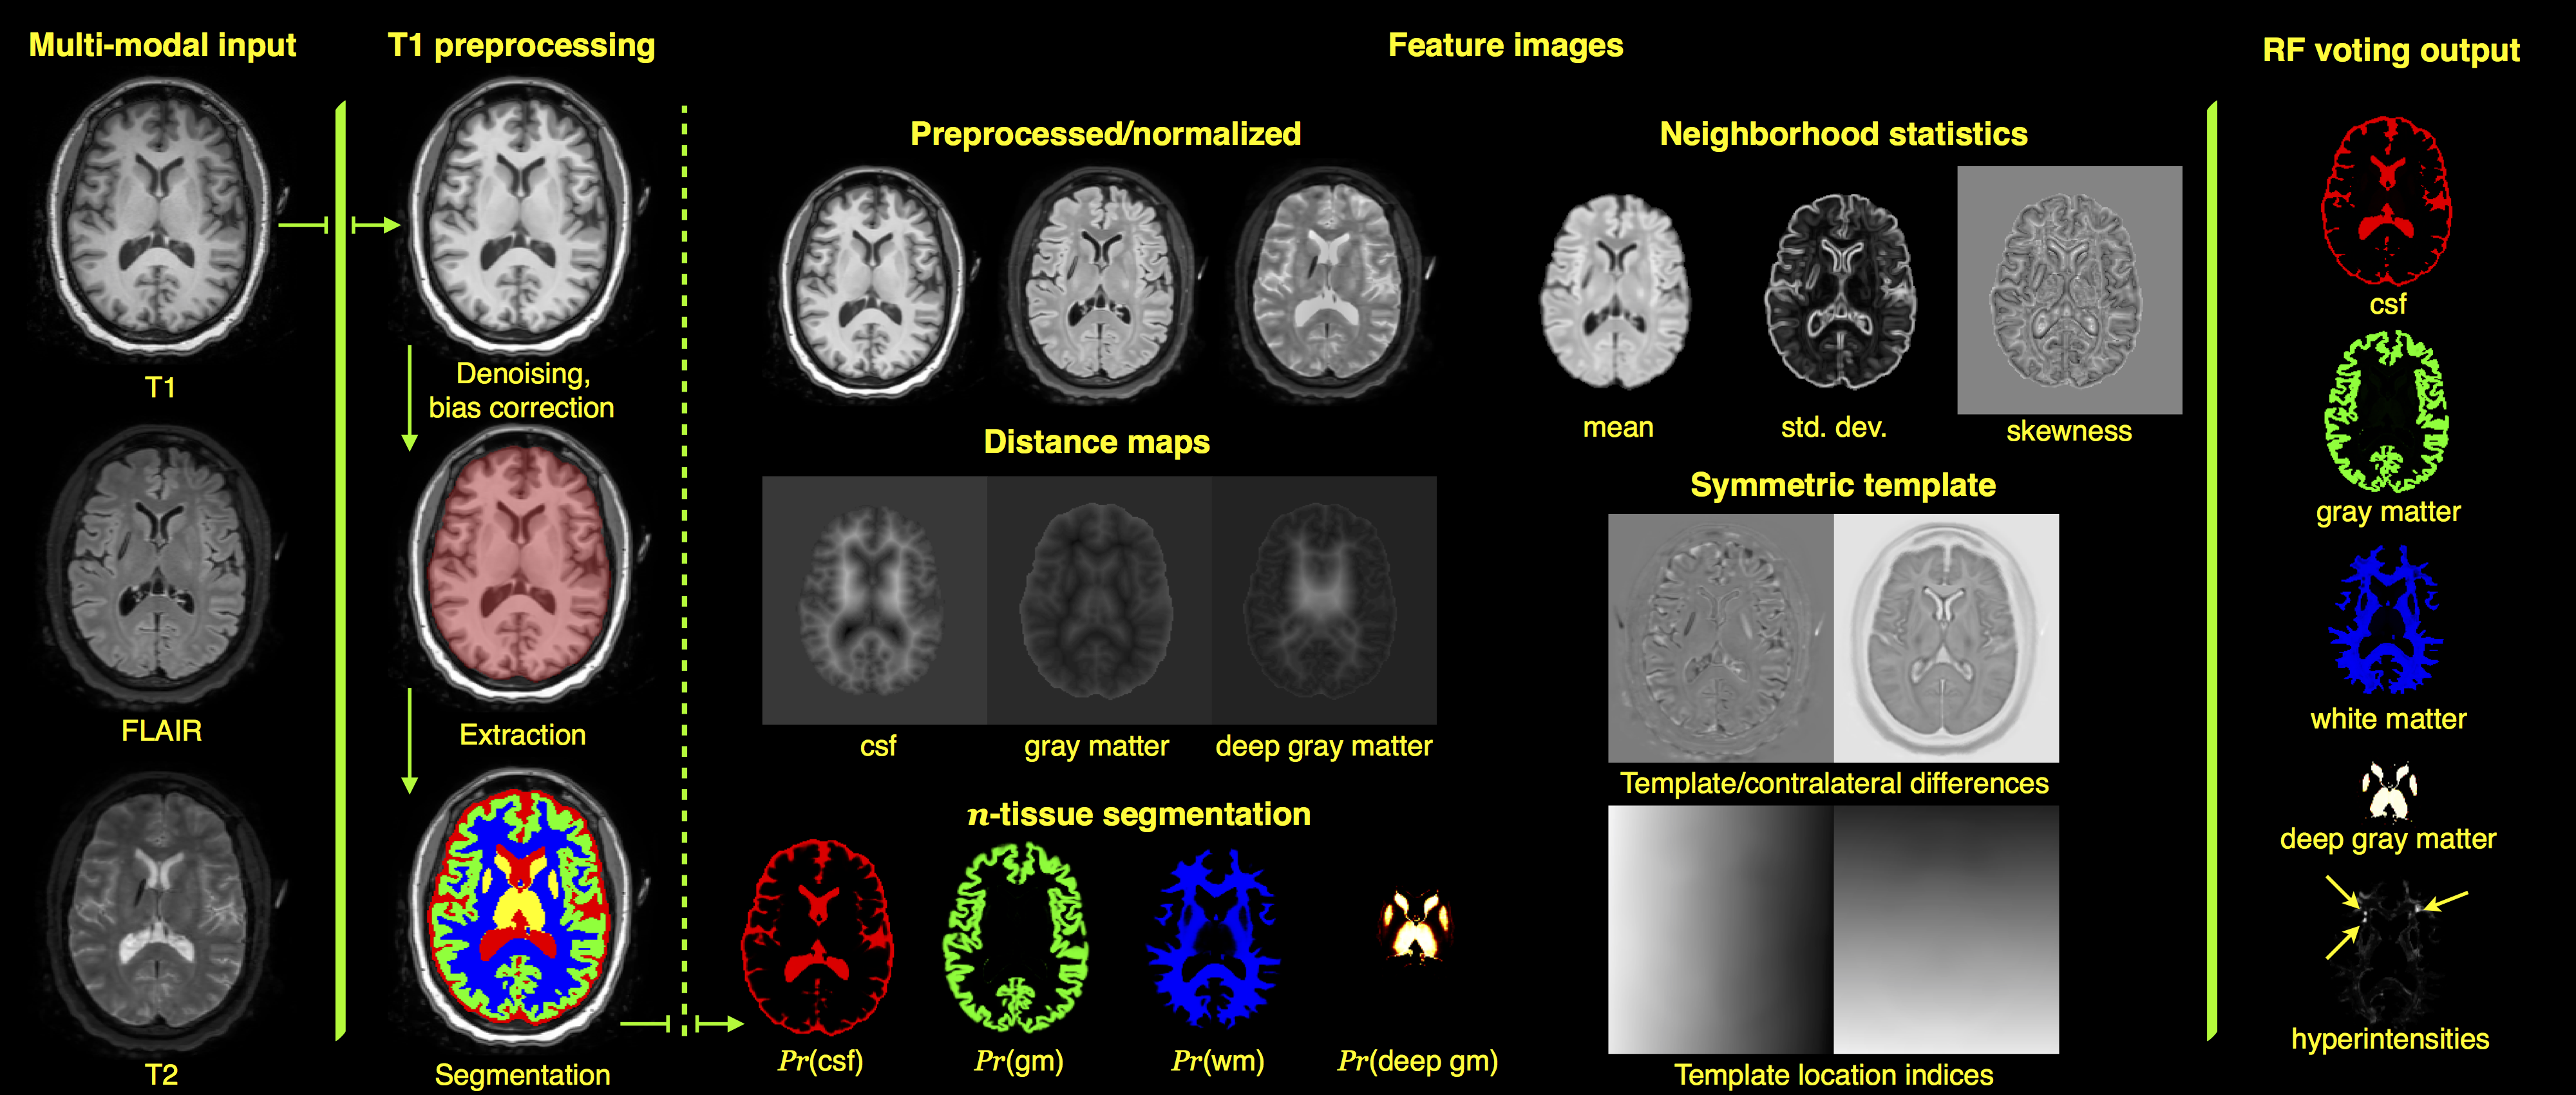
\includegraphics{Figures/featureImages.png}
\caption{Representation of Stage 1 feature images for subject 01C1019.
The FLAIR, T1-, and T2-weighted images are
\added[id=am,remark=NT: no need for 12 dof for
intra-subject normalization]{rigidly} pre-aligned {[}33{]} to the space
of the T1 image. The three modality images are then preprocessed (N4
bias correction {[}34{]} and adaptive denoising {[}35{]}) followed by
application of standard ANTs brain extraction and \(n\)-tissue
segmentation protocols using the MMRR symmetric template and
corresponding priors {[}36{]} applied to the T1 image. The feature
images are then generated for voxelwise input to the RF model which
results in the voting maps illustrated on the right. This gives a
probabilistic classification of tissue type. Not shown are the
probability and voting images for the brain stem and cerebellum.}
\end{figure}

As mentioned previously, input for each subject comprises FLAIR, T1-,
and T2-weighted acquisitions. The FLAIR and T2 images are rigidly
registered to the T1 image using the open-source Advanced Normalization
Tools (ANTs) {[}33{]}. The aligned images are then preprocessed using
the denoising algorithm of {[}35{]} followed by N4 bias correction
{[}34{]} which are then normalized to the intensity range \([0,1]\).
Although we could have used an alternative intensity standardization
algorithm (e.g., {[}37{]}), we found that a simple linear rescaling
produced better results.

\begin{figure}[htbp]
\centering
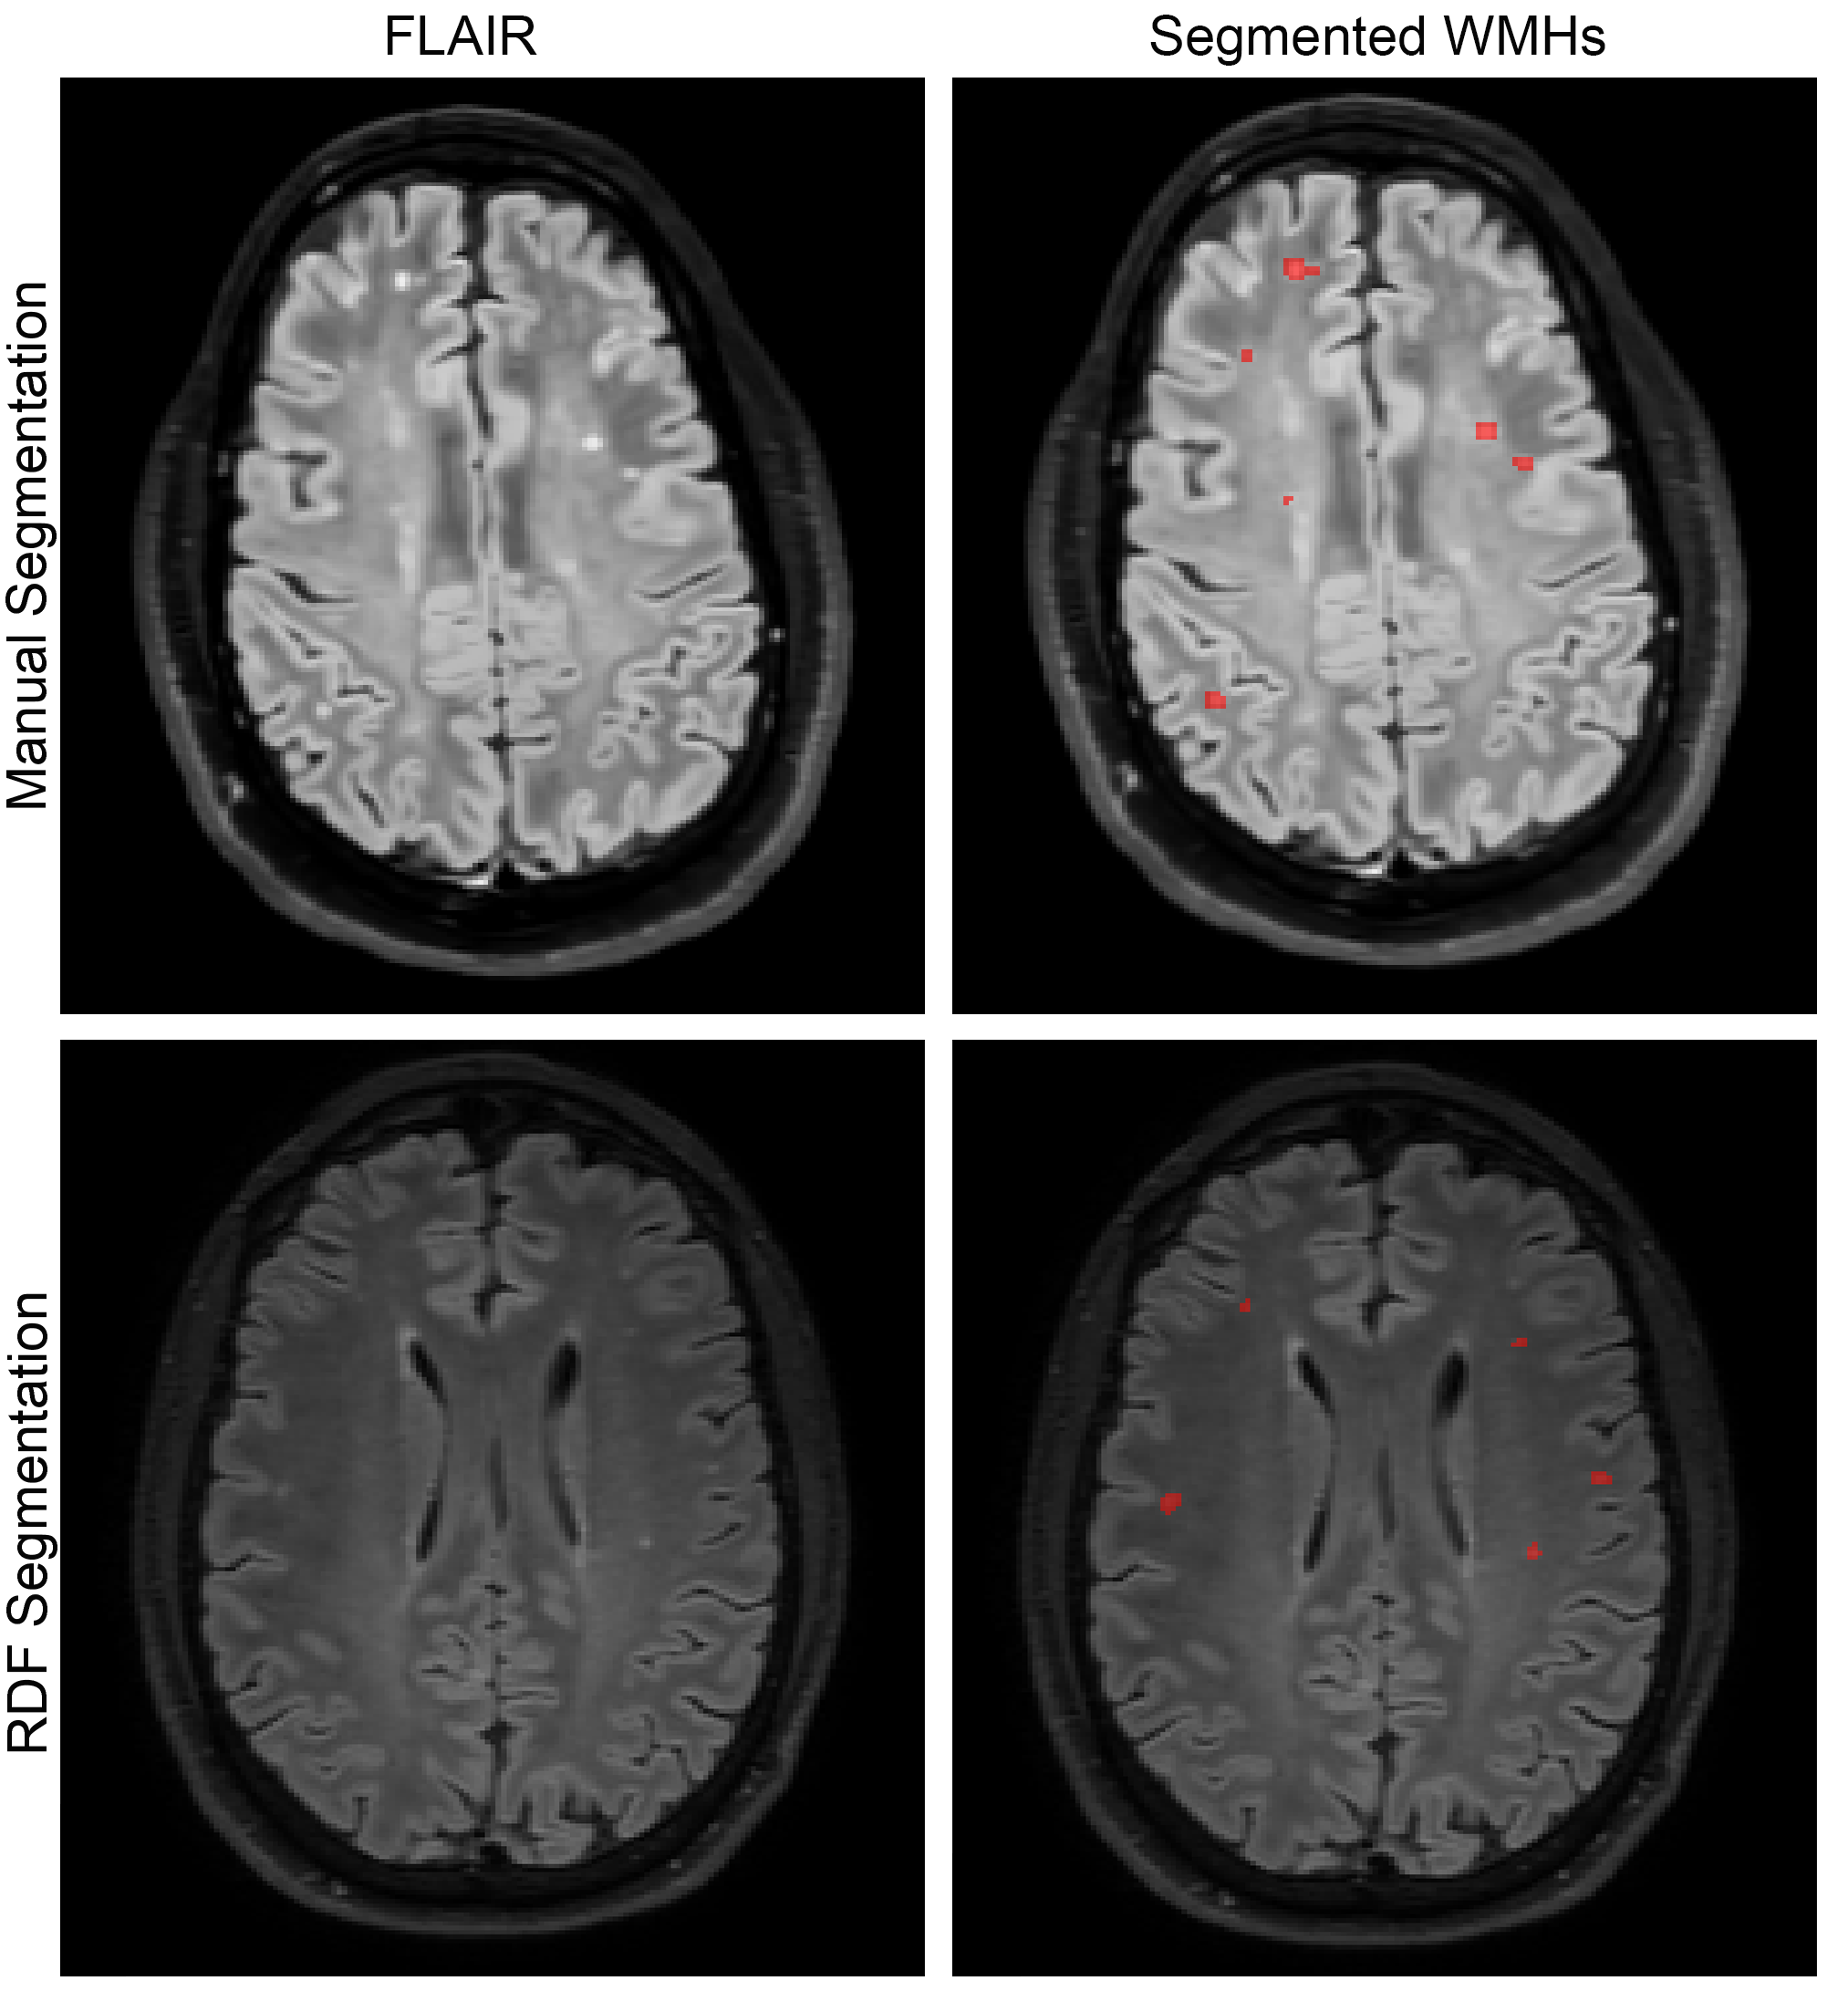
\includegraphics{Figures/montage.png}
\caption{Sample FLAIR acquisition image slices showing both manual (top)
and random forest (RDF) segmentations (bottom) obtained during the
leave-one-out evaluation. Manual segmentations were performed by one of
the authors and provided the ground truth WMH labels for training the
random forest models.}
\end{figure}

The T1 image is then processed via the ANTs brain extraction and normal
tissue segmentation (i.e., the pathology is discounted which is a fairly
safe assumption for the T1 image) protocols as part of the cortical
thickness pipeline described in {[}36{]}.
\added[id=hl]{This protocol involves preprocessing using N4 bias correction followed by a template-based strategy for brain extraction.  Once the
brain has been extracted, we apply a Bayesian-based segmentation algorithm
with a template-based prior probability strategy to segment the
parenchymal tissue types.  The result is} a mask delineating the brain
parenchyma and probabilistic estimates of the cerebrospinal fluid (csf),
gray matter, white matter, deep gray matter, brain stem, and cerebellum.
These provide the expertly annotated labels for the first six tissue
labels given above. The white matter hyperintensities were manually
identified by one of the authors (J. R. S.) using the ITK-SNAP tool
{[}38{]}. Segmentation is performed using the ANTs Atropos tool {[}39{]}
and multi-model optimal symmetric shape/intensity templates {[}26{]}
created from the public MMRR data set {[}40{]} (cf Figure 3).

\begin{figure}[htbp]
\centering
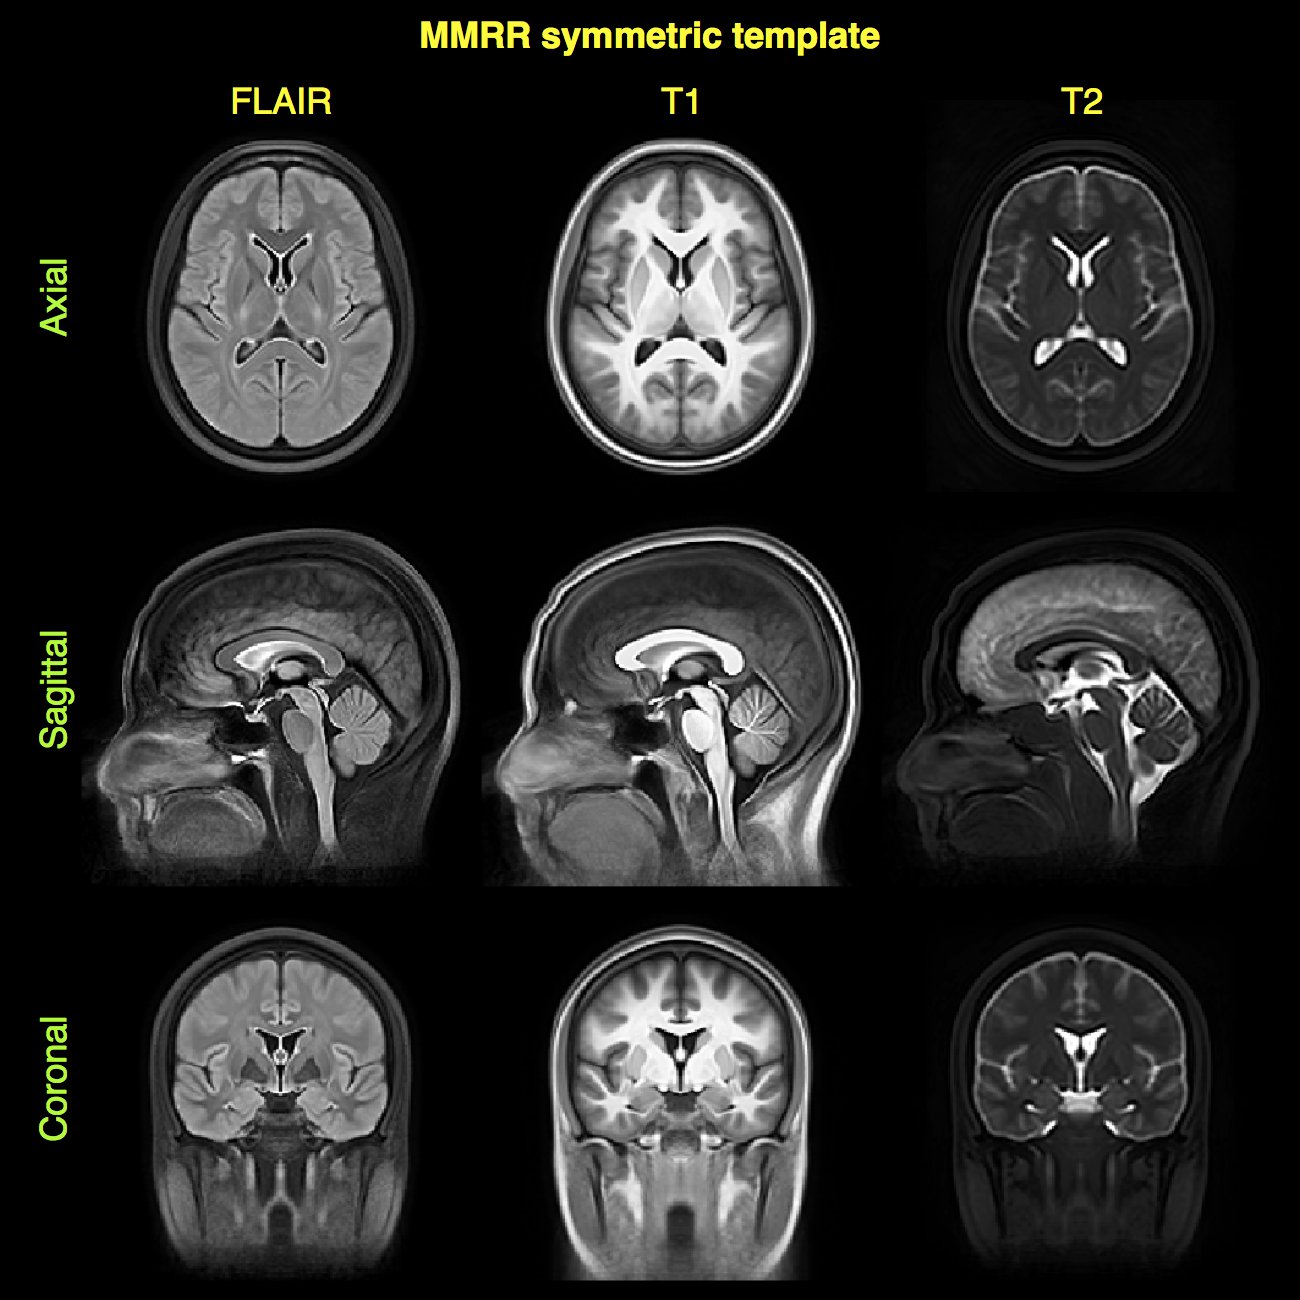
\includegraphics{Figures/MMRR.png}
\caption{Canonical views of the mutlivariate, bilaterally symmetric
template constructed from the MMRR data set {[}40{]} (only shown are the
FLAIR, T1, and T2 modalities--- the components relevant for this work).
Template construction is detailed in {[}26{]}. These images are
important for specific intensity-based features.}
\end{figure}

To model the intensity information the first set of images simply
includes the preprocessed and normalized intensity FLAIR, T1, and T2
image voxel values. We also calculate a set of neighborhood statistics
(mean, standard deviation, and skewness) feature images using a
\added[id=am]{Manhattan} radius of one voxel. For each of the normalized
images, we calculate the difference in intensities with the
corresponding warped template component. Previous success in the
international brain tumor segmentation competition {[}27{]} was based on
an important set of intensity features that were created from
multi-modal templates mentioned previously {[}26{]}. We employ the same
strategy here. For example, the template difference feature image for
the FLAIR image, \(S_{FLAIR}\) is calculated as:

\[S_{FLAIR} - T_{FLAIR}\left(\phi_b^{-1}\right)\]

where \(\phi_b: S \leftrightarrow \underset{b}{\leftrightsquigarrow} T\)
is the transform which maps from the individual subject space to the
template space and \(T_{FLAIR}\) is the FLAIR template component. Also,
to take advantage of the
\added[id=hl,remark=NT:  we are using the "symmetry" of the brain in an analogous sense that if we know the left eye location and color then it is highly probabilistic that we can accurately predict the location and color of the right eye even though a particular face might not be exactly symmetric]{gross}
bilateral symmetry of the normal brain (in terms of both shape and
intensity), and the fact that
\replaced[id=bt]{WMHs do not generally manifest symmetrically across hemispheres}{the presence of WMHs violates that assumption},
we use the symmetric templates to compute the contralateral intensity
differences as an additional intensity feature. For the FLAIR component,
this contralateral difference image is calculated from

\[S_{FLAIR} - S_{FLAIR}\left(\phi_b^{-1}\left(\phi_R\left(\phi_b\right)\right)\right)\]

where \(\phi_R\) denotes a horizontal reflection perpendicular to the
mid-sagittal plane of the symmetric template.

The segmentation probability images described above are used as feature
images to provide a spatial context for the random forest model
prediction step. Additional spatial contextual feature images include
the distance maps {[}41{]} based on the csf, gray matter, and deep gray
matter images. These latter images are intended to help distinguish
white matter hyperintensities from false positives induced by the
partial voluming at the gray/white matter interface. A third set of
images are based on the voxel location within the space of the template.
The T1 image of the subject is registered to the T1 template component
using a B-spline variant {[}42{]} of the well-known ANTs Symmetric
Normalization (SyN) algorithm {[}43{]}. Since the inverse transform is
also derived as part of the registration process, we can warp the voxel
index locations back to the space of the individual subject. Note that
this is similar in motivation to the work of {[}44{]}. However, this
previous work lacks the normalization to the standard coordinate system
provided by the template to dramatically improve spatial specificity
across all subjects.

\subsubsection{Stacked (concatenated) random forests for improved
segmentation
performance}\label{stacked-concatenated-random-forests-for-improved-segmentation-performance}

In previous brain tumor segmentation work {[}26{]}, it was demonstrated
that a concatenated supervised approach, whereby the prediction output
from the first random forest model serves as partial input for a second
random forest model, can significantly improve segmentation performance.
We do the same thing for the work described here
\added[id=lw]{where we employ two stacked random forests (or two "stages")}.
The Stage 1 feature images of the training data (as described
previously) are used to construct the Stage 1 model. The training data
Stage 1 features are then used to produce the voxelwise
\added[id=lw]{"voting maps" (i.e., the classification count of each decision tree for each tissue label)}
via the Stage 1 random forest model. All the Stage 1 features plus the
Stage 1 voting maps are used as input to the Stage 2 model. In addition,
we use the Stage 1 voting maps as tissue priors
\added[id=lw]{(i.e., probabilistic estimates of the tissue spatial locations)}
for a second application of the Atropos maximum aposteriori algorithm
with an additional Markov Random Field spatial prior (MAP-MRF) {[}39{]}.
However, for the second stage we use all three aligned preprocessed
images for a multivariate segmentation. The resulting seven posterior
probability images constitute a third additional feature image set for
Stage 2.

\subsubsection{Code and data
availability}\label{code-and-data-availability}

As pointed out in a recent comprehensive multiple sclerosis lesion
segmentation review {[}45{]}, although the number of algorithms reported
in the literature is quite extensive, there were only four publicly
available segmentation algorithms at the time of writing of which none
are based on supervised learning. As we did for our brain tumor
segmentation algorithm {[}26{]}, all of the code described in this work
is publicly available through the open-source ANTs/ANTsR toolkits.
Through ANTsR (an add-on toolkit which, in part, bridges ANTs and the R
statistical project) we use the \texttt{randomForest} package {[}46{]}
using the default settings with 2000 trees per model and 500 randomly
selected samples per label per image.
\added[id=bt]{Note that we saw little variation in performance when these parameters were changed which is consistent with our previous experience.}

In addition, similar to our previous offering,\footnote{\url{https://github.com/ntustison/ANTsAndArboles}}
we plan on creating a self-encapsulated example to showcase the proposed
methodology. The fact that the data will also be made available through
the FITBIR repository along with the manual labelings will facilitate
reproducibility on the part of the reader as well as any interest in
extending the proposed framework to other data sets.

\subsubsection{Evaluation protocol
overview}\label{evaluation-protocol-overview}

In order to evaluate the protocol described, we performed a
leave-one-out evaluation using the data acquired from the 24 subjects
described above. Initial processing included the creation of all Stage 1
feature images for all subjects. The initial brain segmentation of each
T1 image and the manual white matter hyperintensity tracings were
combined to provide the truth labels for the training data. The
``truth'' labels are the seven anatomical regions given above.

The leave-one-out procedure is as follows:

\begin{itemize}
\tightlist
\item
  Create Stage 1 feature images for all 24 subjects.
\item
  For each of the 24 subjects:

  \begin{itemize}
  \tightlist
  \item
    sequester the current subject and corresponding feature images.
  \item
    construct the Stage 1 random forest model from the remaining 23
    subjects.
  \item
    apply the Stage 1 random forest model to the feature images of the
    23 training subjects.
  \item
    the previous step produces the Stage 1 voting maps for all seven
    labels.
  \item
    for each of the 23 subjects, perform a Bayesian-based segmentation
    with an MRF spatial prior using the seven voting maps are used as
    additional tissue priors.
  \item
    construct the Stage 2 random forest model from all the Stage 1
    feature images, seven voting maps, and seven posterior probability
    maps from the previous step.
  \item
    send the sequestered subject through the random forest models for
    both stages.
  \item
    compare the final results with the manually-defined white matter
    hyperintensity regions.
  \end{itemize}
\end{itemize}

\section{Results}\label{results}

\subsection{Ranking feature
importance}\label{ranking-feature-importance}

After performing the leave-one-out evaluation described at the end of
the previous section, we calculated the \texttt{MeanDecreaseAccuracy}
feature values for each of the 24 subjects \(\times\) 2 models per
subject \(=48\) total models. This measure (per feature, per model) is
calculated during the out-of-bag phase of the random forest model
construction and quantifies the decrease in prediction accuracy from
omitting the specified feature. In other words, this quantity helps
determine the importance of a particular feature and, although we save
such efforts for future work, this information provides us with guidance
for future feature pruning and/or additions.

\begin{figure}[htbp]
\centering
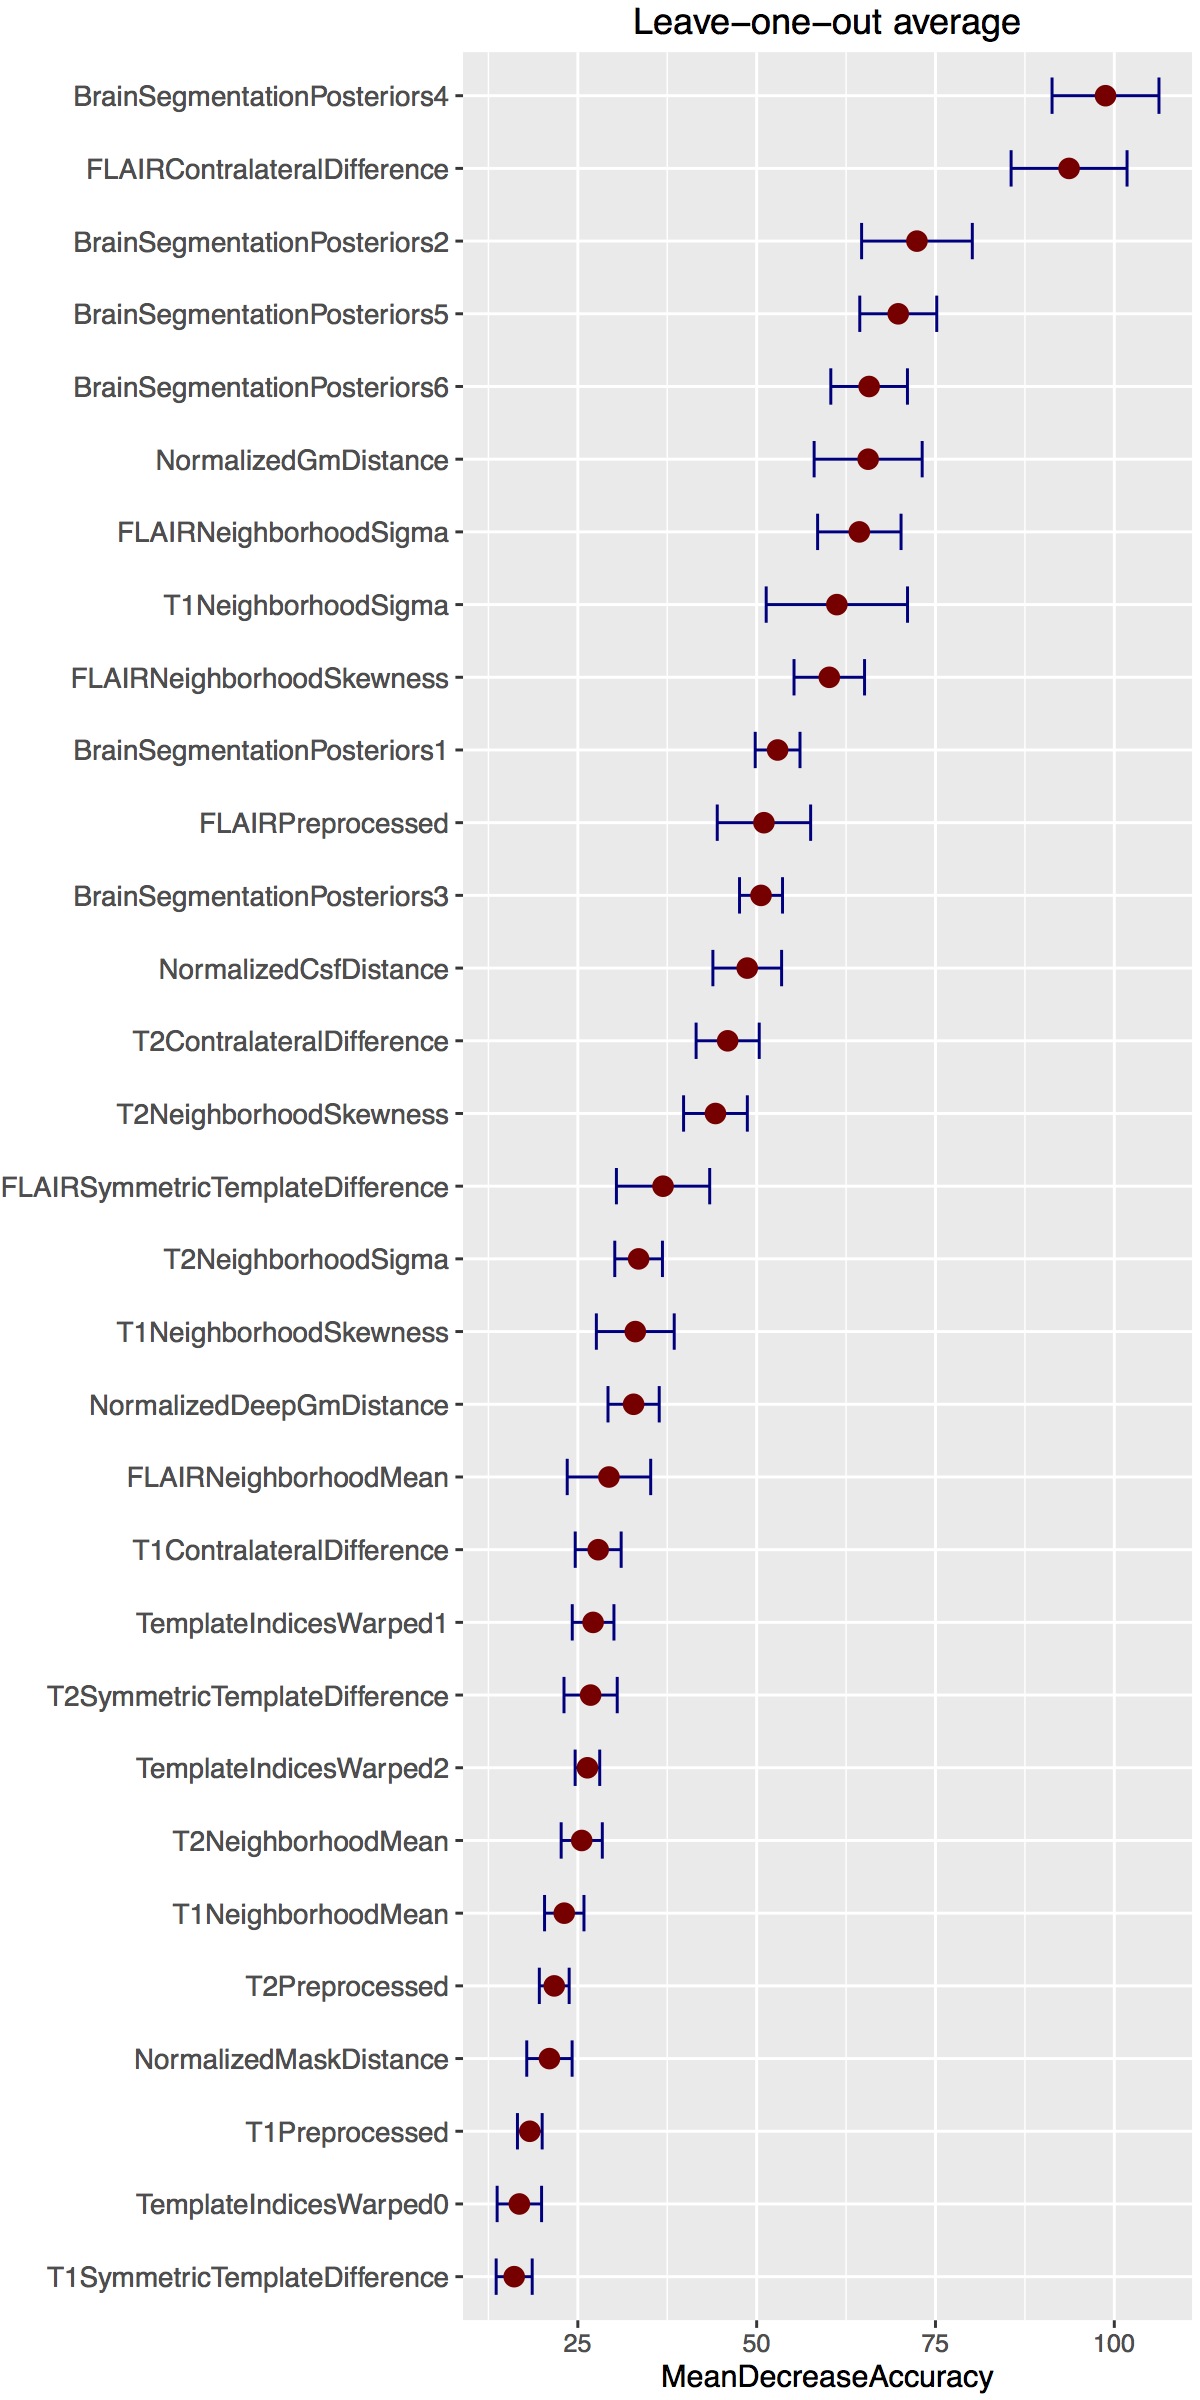
\includegraphics{Figures/averageLeaveOneOutStage1.png}
\caption{Average \texttt{MeanDecreaseAccuracy} plots generated from the
creation of all 24 random forest models for Stage 1 during the
leave-one-out evaluation. These plots are useful in providing a
quantitative assessment of the predictive importance of each feature.
\added[id=nt]{Features are ranked in descending order of importance.}
The horizontal error bars provide the \(95^{th}\) percentile
\deleted[id=bt]{(i.e., $1.96 \times \sigma$)} and illustrate the
stability of the feature importance across the leave-one-out models.
\added[id=nt]{At this initial stage only 31 features images are used.}}
\end{figure}

\begin{figure}[htbp]
\centering
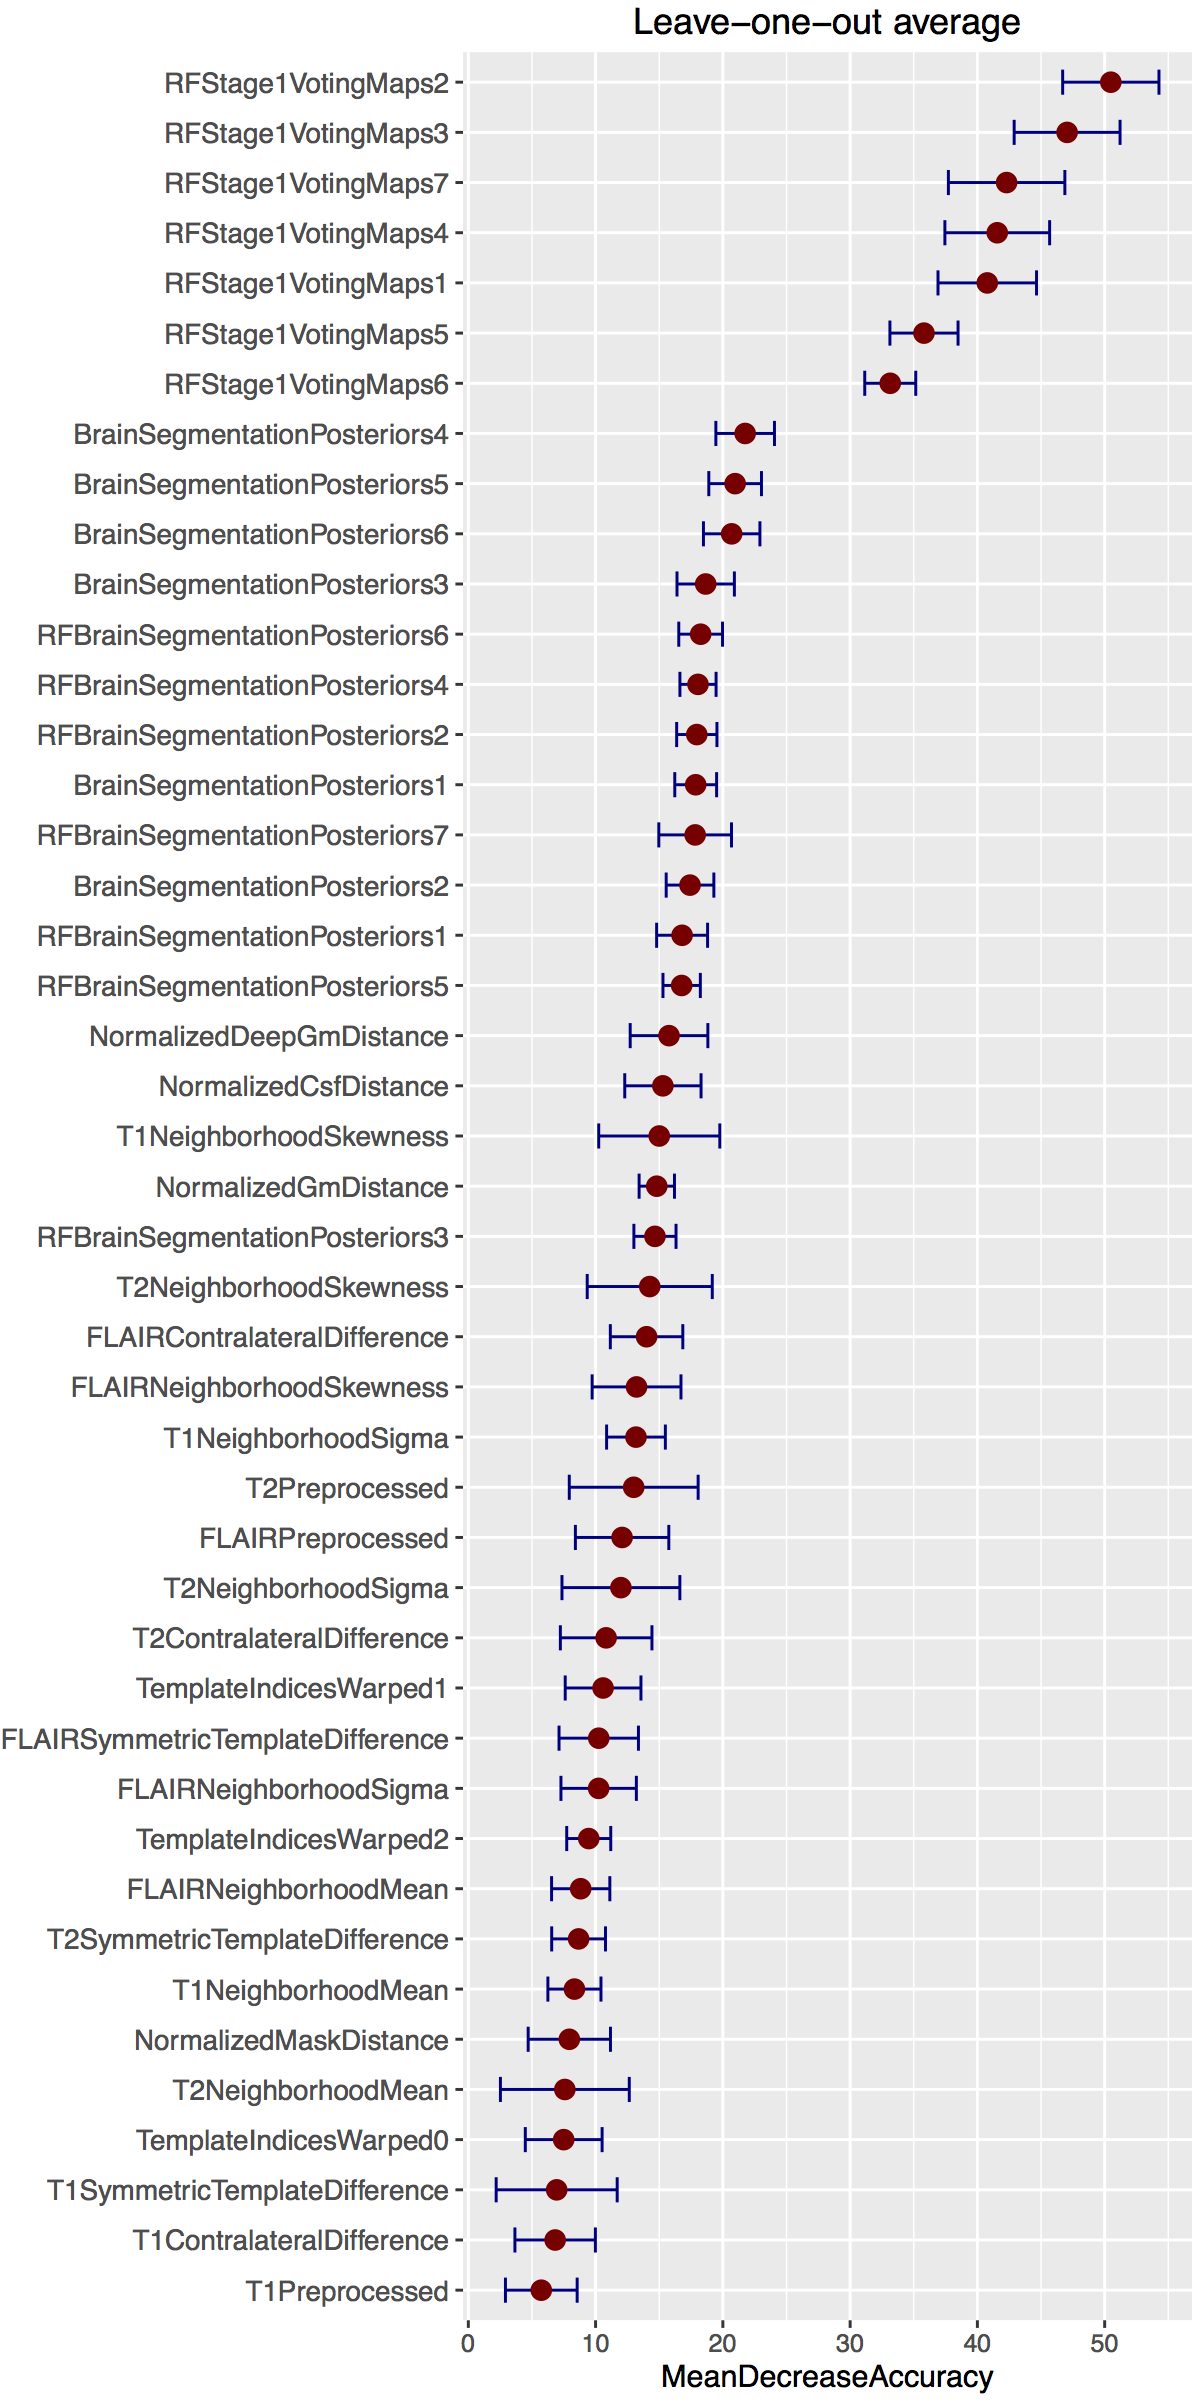
\includegraphics{Figures/averageLeaveOneOutStage2.png}
\caption{Average \texttt{MeanDecreaseAccuracy} plots generated from the
creation of all 24 random forest models for Stage 2 during the
leave-one-out evaluation. These plots are useful in providing a
quantitative assessment of the predictive importance of each feature.
\added[id=nt]{Features are ranked in descending order of importance.}
The horizontal error bars provide the \(95^{th}\) percentile
\deleted[id=bt]{(i.e., $1.96 \times \sigma$)} and illustrate the
stability of the feature importance across the leave-one-out models.
\added[id=nt]{We augment the 31 feature images from the first stage by adding an additional
7 voting maps and 7 segmentation posteriors from application of the Bayesian-based
segmentation for a total of 45 images for the second stage.}}
\end{figure}

The resulting rankings for both Stages are given in Figures 4 and 5
where the values for the separate stages are averaged over the entire
corresponding model set. In addition, we track the variance for each
feature over all models to illustrate the stability of the chosen
features during the evaluation. This latter information is illustrated
as horizontal errors bars providing the \(95^{th}\) percentile
\deleted[id=bt]{(i.e., $1.96 \times \sigma$)}. Note that the reader can
cross reference Table 1 for identifying corresponding feature types and
names.

One can also use these measurements as a type of sanity check. For
example, from the Stage 1 plot, one can see that the
\texttt{MeanDecreaseAccuracy} values for the location indices in the
anterior-posterior direction (i.e., \texttt{TemplateIndicesWarped1}) are
greater than those for either the inferior-superior (i.e.,
\texttt{TemplateIndicesWarped0}) or the left-right (i.e.,
\texttt{TemplateIndicesWarped0}) directions in the space of the
symmetric template.
\deleted[id=bt]{This is intuitive since, as discussed previously, manifestation of TBI white
matter hyperintensities can often be confused with higher intensities at the
periventricular caps in normal subjects [@Neema:2009aa]}
\deleted[id=am]{whereas there does not seem to
be contralateral bias in manifestation of white matter hyperintensities in TBI.}

Additionally, it is interesting to note some of the other top performing
features for Stage 1. The contralateral difference FLAIR image is highly
discriminative over the set of evaluation random forest models
\added[id=bt]{(see Figure 6)}. This accords with the known clinical
relevance of FLAIR images for identifying white matter hyperintensities
and the fact that such pathology does not \added[id=nt]{typically}
manifest symmetrically in both hemispheres. Interestingly, the posterior
maps for the deep gray matter are extremely important for accurate white
matter hyperintensity segmentation. Perhaps the spatial specification of
deep gray matter aids in the removal of false positives. Inspection of
the bottom of the plots demonstrates the lack of discriminating features
associated with the T1 image which is also well-known in the clinical
literature.

\begin{figure}[htbp]
\centering
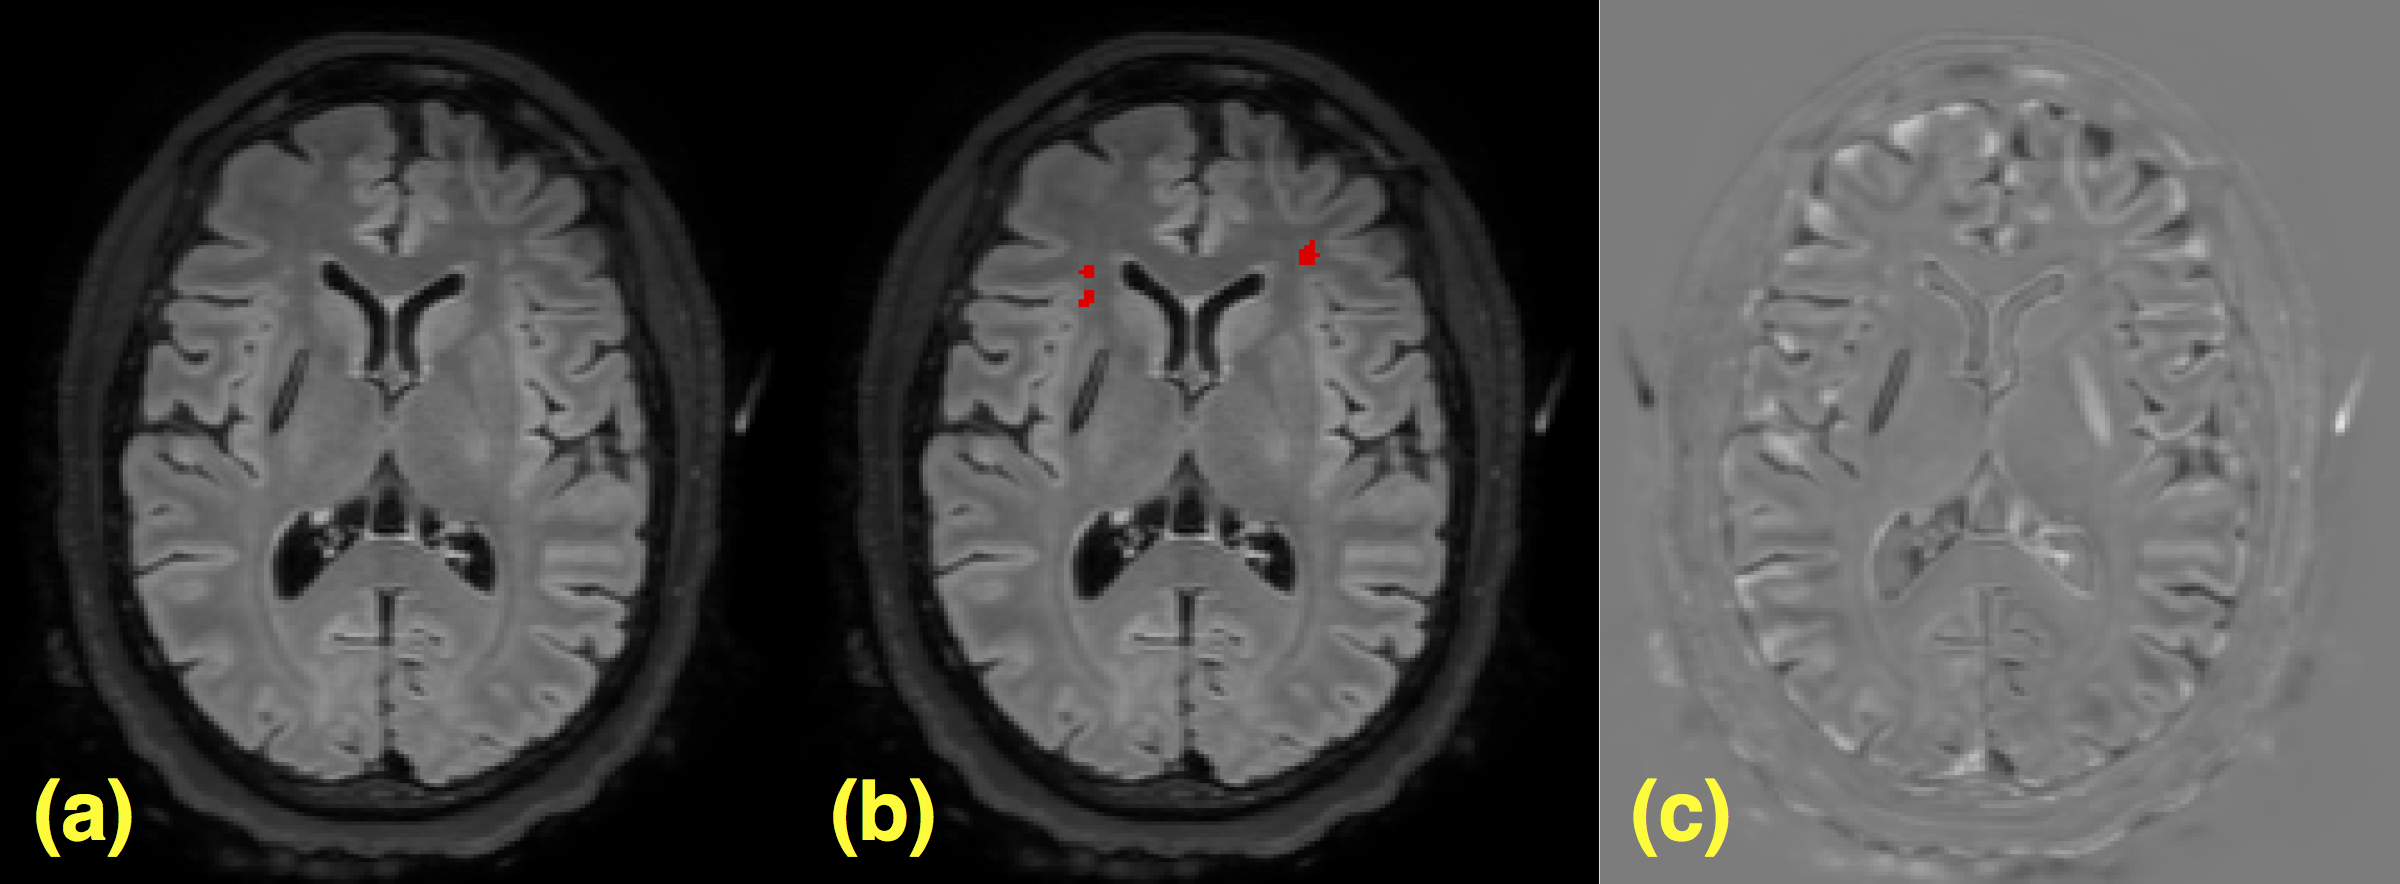
\includegraphics{Figures/FLAIRcontralaleteralWithLesions.png}
\caption{\added[id=nt]{(a) FLAIR image slice illustrating WMHs which have been manually delineated
in (b).  (c) Contralateral FLAIR difference image.}}
\end{figure}

As described earlier, for Stage 2, we used the output random forest
voting maps from Stage 1 as both features themselves and as priors for
input to a Bayesian-based segmentation with an additional MRF spatial
prior. In Figure 5, the voting maps are labeled as
``\texttt{RFStage1VotingMaps}'' where the final numeral is associated
with the brain parenchymal labeling given previously. Similarly, the
additional RF prior segmentation feature probability maps are labeled as
``\texttt{RFBrainSegmentationPosteriors}''. The Stage 2 feature
importance plot follows similar trends as that for Stage 1 with the T1
images not contributing much to the identification of white matter
hyperintensity voxels. The initial voting maps from Stage 1 are
extremely important with the top 3 being the estimated locations of the
1) gray matter, 2) white matter, and 3) white matter hyperintensities.
Since these tissue type can be conflated based on intensity alone it is
intuitive that such features would be important.

\subsection{White matter hyperintensity segmentation
evaluation}\label{white-matter-hyperintensity-segmentation-evaluation}

In Figure 7 are the segmentation comparisons derived from manual
segmentations of the same data. Despite the large variability
characteristic with manual labelings in related fields {[}45, 47, 48{]},
such labelings are characteristic of current clinical practices and the
methodology proposed herein is readily adapted to refinements in
training data. On the left of Figure 7 are the improvement in Dice
values {[}49{]}, \added[id=nt]{i.e.,}

\[ Dice = 2 \frac{\sum_r|S_r \cap T_r|}{\sum_r|S_r| + |T_r] } \]

\added[id=nt]{over all white matter hyperintensities when comparing the segmentations between the two stages
where the sum is taken over all individually labeled manual, $T_r$, and automated, $S_r$, lesions and $\cap$
represents the intersection between the manual/automated lesion pair.}
Performing the second round of supervised learning improves these Dice
values. One can also note from the right side of Figure 6 that the total
lesion load volume illustrates a few subjects that are severe outliers
in terms of the number of false positives. The second round helps to
correct this issue.

\begin{figure}[htbp]
\centering
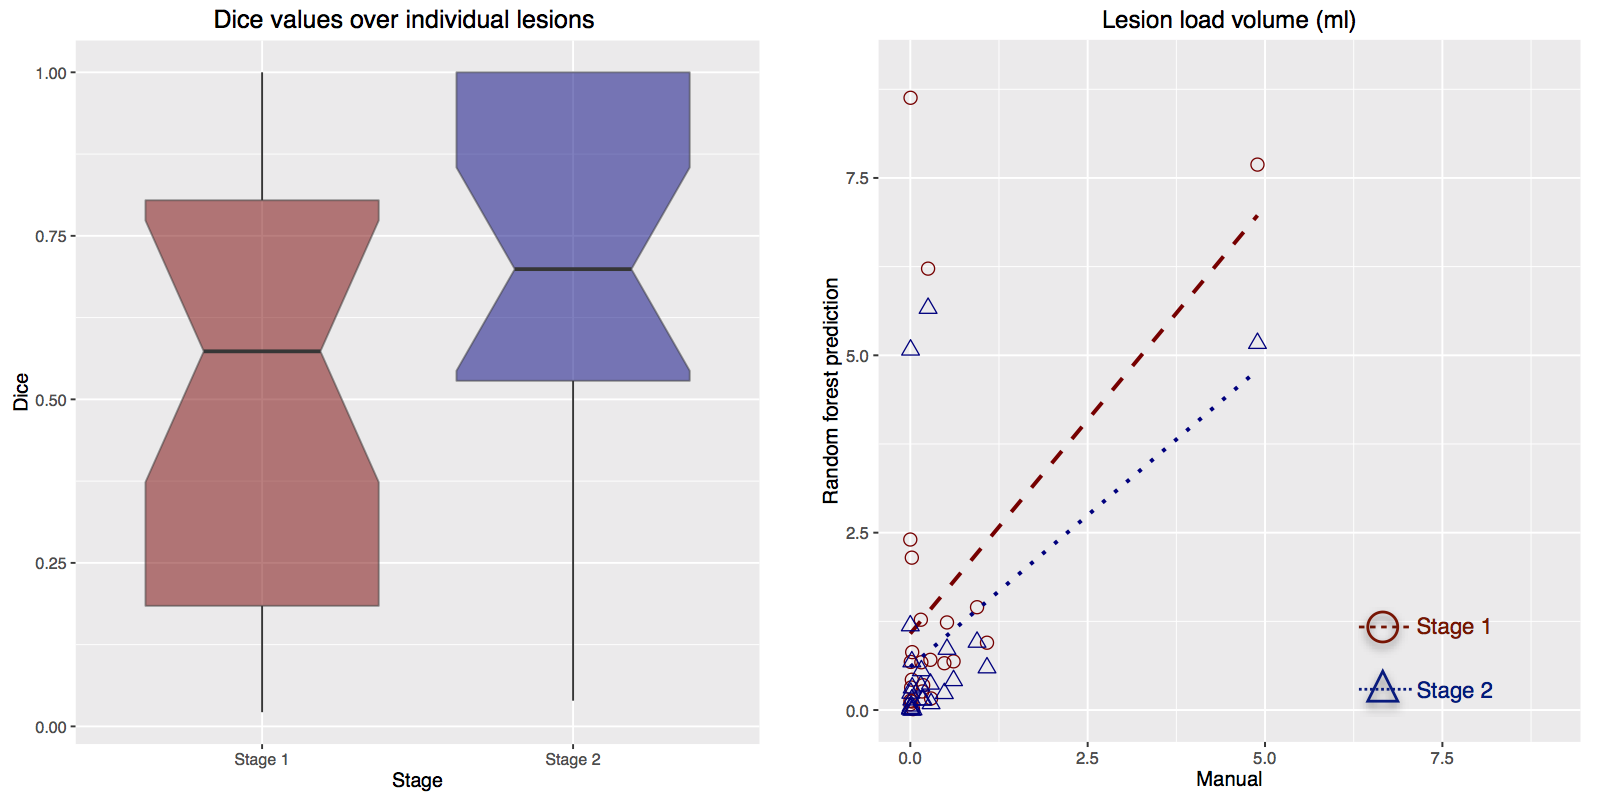
\includegraphics{Figures/llvAndDice.png}
\caption{Comparison with manual delineation of white matter
hyperintensities. On the left are the calculate Dice values over all
white matter hyperintensities. Note the improvement in the Dice metric
from the employment of the Stage 2 component of the processing pipeline.
(Right) Similar results can be seen by comparing the total lesion load
volume between manual and automated detection strategies. Although some
outliers are found after the Stage 2 processing in a couple subjects,
the number of outliers caused by false positives is significantly with
the second stage processing.}
\end{figure}

\section{Discussion}\label{discussion}

The current communications describes a supervised statistical learning
methodology for identifying WHMs within multimodal MR brain imaging.
This effort utilized information acquired from the manual segmentation
of WMHs from FLAIR images to help build two-stage ensembles of decision
trees for the automated identification of these lesions. Although only a
single expert was used to produce the manual labelings, our intent is to
further refine the proposed paradigm by crowdsourcing with feedback from
other experts who interact with both the data and methodology. Also, we
recognize that only a single site was used for evaluating the proposed
framework. However, we are currently processing other site data with the
models developed for this work and the results look promising since the
developed features are site-agnostic.

As far as we know, this is the first report utilizing a novel random
forest approach to identify WMHs in a cohort of TBI patients. TBI WMHs
tend to be more difficult to segment than MS lesions as the former tend
to be smaller with an overall smaller lesion load. Also, enhancement
protocols with the former tend to be less successful than with the
latter. As mentioned previously, the work in MS lesion segmentation is
extensive with a handful of techniques being publicly available. Our
framework is also available as open-source as part of well-known
neuroimaging tools which easily allows for additions/extensions but is
also, as far as we know, the first random forest-based technique
available for such application.

Two major meta-analyses of WMHs have been published covering the periods
of 1966-2009 and 2010-2015, respectively. The earlier meta-analysis
covered 53 longitudinal studies that included samples of high-risk
populations, i.e., patients selected for a specific disease or condition
such as hypertension, whereas other studies recruited samples of the
general population. Longitudinal studies of samples representative of
the general population are more relevant to the focus of the present
paper. Debette \& Markus {[}9{]} found that the presence of WMHs was
related to subsequent cognitive decline, a higher risk of developing
dementia, stroke, and of mortality. Lesion volume at baseline was also
predictive of cognitive decline. Limitations of this meta-analysis
include heterogeneity in the method of measuring WMHs; some studies used
automated volumetric measurement, whereas others used a visual rating
scale. The studies analyzed by Debette \& Markus were limited to the
occurrence of one of the aforementioned conditions which they analyzed
by hazard ratios.

A recent meta-analysis by Kloppenborg et al. {[}10{]} of 23
cross-sectional studies reporting MRI and concurrent neuropsychological
results in patients with heterogeneous diagnoses but without previously
diagnosed cognitive impairment, found that WMHs were associated with
cognitive deficit (effect size of -0.10, 95\% CI: -0.13 to -0.08) after
controlling for age. These studies also differed in the metric used to
measure the WMHs, including volume, \% of total intracranial volume, and
a visual rating score. The effect size for the association with
cognitive deficit in these cross-sectional studies did not differ
significantly across various cognitive domains or the method of
measuring lesion volume. Among eight longitudinal studies analyzed by
Kloppenborg et al that included a follow-up MRI and also controlled for
age, the effect size for the association of progression in WMHs and
cognitive impairment was -0.16 (95\% CI:-0.27 to -0.09). This
association was stronger for attention and executive function than for
memory and processing speed. Although baseline WMHs were predictive of
cognitive deficit at follow-up in the seven studies which did not repeat
MRI, the effect size was smaller {[}-0.10 (95\% CI: 0.13 to -0.05) than
in the longitudinal studies that calculated progression in WMHs. In
summary, progression of WMHs seen on repeat MRI has a stronger relation
to cognitive deficit than concurrent imaging findings. These
meta-analyses support the rationale for repeating an MRI in patients
younger than 50 years whose initial scan shows WMHs. Despite the
above-described associations between WMHs, cognitive decline, increased
risk of developing dementia, and mortality, these lesions receive little
attention in current clinical workflows. When reported in a standard
neuroradiologist interpretation, they are typically handled as
incidental findings and are assigned little clinical significance. This
likely reflects the impracticality of performing a detailed assessment
of number, volume, and distribution within a qualitative
neuroradiologist interpretation as well as the lack of correlative
information on how the presence and distribution of these lesions may
inform a diagnosis and prognosis in the appropriate clinical setting. To
date, automated or semi-automated tools for the detection of WMHs have
lacked the specificity and efficiency for the mining of large-scale
datasets to generate highly granular data on whether these lesions
possess any true diagnostic or prognostic value in the setting of a
specific disease process. The present communication describes a
supervised statistical learning tool that is appropriate for the
application to such large-scale datasets.

The currently described tool is just one example of how ``deep
learning'' algorithms might be applied to aid in the diagnosis of TBI
and other disease processes through the specific identification of
features predictive of a given disease state. It is an important
demonstration of the potential power of these analytical approaches in
the rapid but comprehensive mining of information from neuroimaging
examinations. Deep learning algorithms are presently employed across a
wide variety of settings for the rapid identification of predictive
imaging features. Automobile manufacturers utilize these types of
approaches to equip self-driving vehicles to recognize and respond to
unique external surroundings through the identification of visual
information sufficiently similar to previously assimilated training
data. Similarly, in the context of the neuroimaging assessments, deep
learning approaches may allow for the rapid identification of
information predictive of disease state in an individual patient. These
approaches may be applied to the identification of macroscopically
visible lesions as described in the current communication. Additionally,
these approaches might be applied to the interrogation of imaging data
in the individual patient with a primary quantitative output metrics to
include sequences such as diffusion tensor imaging (DTI) and its
variants, functional connectivity, perfusion weighted imaging, and
cortical thickness assessments. At present, these sequences are confined
to cohort-based research studies due to the lack of available analytical
tools to assess the information in the setting of the individual
patient. Application of deep learning approaches in the context of data
with primary quantitative outputs will require large scale normative and
disease specific databases. Acquisition of these data is resource
intensive and requires a multi-center approach with harmonized scanner
between sites and correlative non-imaging clinical data. Large scale TBI
data is becoming increasingly available through activities such as the
Chronic Effects of Neurotrauma Consortium (CENC), Transforming Research
and Clinical Knowledge in TBI (TRACK-TBI), Collaborative European
Neurotrauma Effectiveness Research in TBI (CENTER-TBI), Department of
Defense Alzheimer's Disease Neuroimaging Initiative (DOD-ADNI), and
other data being consolidated through the Federal Interagency TBI
repository (FITBIR). In concert with any available high quality
normative neuroimaging data, deep learning algorithms may be well
positioned to help transform how neuroimaging is interpreted for the
clinical management of patients with this disease process.

\clearpage

\listofchanges

\clearpage

\section*{References}\label{references}
\addcontentsline{toc}{section}{References}

\hypertarget{refs}{}
\hypertarget{ref-Bigler:2013aa}{}
1. Bigler, E. D., Abildskov, T. J., Petrie, J., Farrer, T. J., Dennis,
M., Simic, N., Taylor, H. G., Rubin, K. H., Vannatta, K., Gerhardt, C.
A., Stancin, T., and Owen Yeates, K. ``\textbf{Heterogeneity of Brain
Lesions in Pediatric Traumatic Brain Injury}'' \emph{Neuropsychology}
27, no. 4 (2013): 438--51.
doi:\href{https://doi.org/10.1037/a0032837}{10.1037/a0032837}

\hypertarget{ref-Smitherman:2016aa}{}
2. Smitherman, E., Hernandez, A., Stavinoha, P. L., Huang, R., Kernie,
S. G., Diaz-Arrastia, R., and Miles, D. K. ``\textbf{Predicting Outcome
After Pediatric Traumatic Brain Injury by Early Magnetic Resonance
Imaging Lesion Location and Volume}'' \emph{J Neurotrauma} 33, no. 1
(2016): 35--48.
doi:\href{https://doi.org/10.1089/neu.2014.3801}{10.1089/neu.2014.3801}

\hypertarget{ref-Marquez-de-la-Plata:2007aa}{}
3. Marquez de la Plata, C., Ardelean, A., Koovakkattu, D., Srinivasan,
P., Miller, A., Phuong, V., Harper, C., Moore, C., Whittemore, A.,
Madden, C., Diaz-Arrastia, R., and Devous, M., Sr. ``\textbf{Magnetic
Resonance Imaging of Diffuse Axonal Injury: Quantitative Assessment of
White Matter Lesion Volume}'' \emph{J Neurotrauma} 24, no. 4 (2007):
591--8.
doi:\href{https://doi.org/10.1089/neu.2006.0214}{10.1089/neu.2006.0214}

\hypertarget{ref-Moen:2014aa}{}
4. Moen, K. G., Brezova, V., Skandsen, T., Håberg, A. K., Folvik, M.,
and Vik, A. ``\textbf{Traumatic Axonal Injury: The Prognostic Value of
Lesion Load in Corpus Callosum, Brain Stem, and Thalamus in Different
Magnetic Resonance Imaging Sequences}'' \emph{J Neurotrauma} 31, no. 17
(2014): 1486--96.
doi:\href{https://doi.org/10.1089/neu.2013.3258}{10.1089/neu.2013.3258}

\hypertarget{ref-Ding:2008aa}{}
5. Ding, K., Marquez de la Plata, C., Wang, J. Y., Mumphrey, M., Moore,
C., Harper, C., Madden, C. J., McColl, R., Whittemore, A., Devous, M.
D., and Diaz-Arrastia, R. ``\textbf{Cerebral Atrophy After Traumatic
White Matter Injury: Correlation with Acute Neuroimaging and Outcome}''
\emph{J Neurotrauma} 25, no. 12 (2008): 1433--40.
doi:\href{https://doi.org/10.1089/neu.2008.0683}{10.1089/neu.2008.0683}

\hypertarget{ref-Pierallini:2000aa}{}
6. Pierallini, A., Pantano, P., Fantozzi, L. M., Bonamini, M., Vichi,
R., Zylberman, R., Pisarri, F., Colonnese, C., and Bozzao, L.
``\textbf{Correlation Between MRI Findings and Long-Term Outcome in
Patients with Severe Brain Trauma}'' \emph{Neuroradiology} 42, no. 12
(2000): 860--7.

\hypertarget{ref-Weiss:2008aa}{}
7. Weiss, N., Galanaud, D., Carpentier, A., Tezenas de Montcel, S.,
Naccache, L., Coriat, P., and Puybasset, L. ``\textbf{A Combined
Clinical and MRI Approach for Outcome Assessment of Traumatic Head
Injured Comatose Patients}'' \emph{J Neurol} 255, no. 2 (2008): 217--23.
doi:\href{https://doi.org/10.1007/s00415-008-0658-4}{10.1007/s00415-008-0658-4}

\hypertarget{ref-Levin:1988aa}{}
8. Levin, H. S., Williams, D., Crofford, M. J., High, W. M., Jr,
Eisenberg, H. M., Amparo, E. G., Guinto, F. C., Jr, Kalisky, Z., Handel,
S. F., and Goldman, A. M. ``\textbf{Relationship of Depth of Brain
Lesions to Consciousness and Outcome After Closed Head Injury}'' \emph{J
Neurosurg} 69, no. 6 (1988): 861--6.
doi:\href{https://doi.org/10.3171/jns.1988.69.6.0861}{10.3171/jns.1988.69.6.0861}

\hypertarget{ref-Debette:2010aa}{}
9. Debette, S. and Markus, H. S. ``\textbf{The Clinical Importance of
White Matter Hyperintensities on Brain Magnetic Resonance Imaging:
Systematic Review and Meta-Analysis}'' \emph{BMJ} 341, (2010): c3666.

\hypertarget{ref-Kloppenborg:2014aa}{}
10. Kloppenborg, R. P., Nederkoorn, P. J., Geerlings, M. I., and Berg,
E. van den. ``\textbf{Presence and Progression of White Matter
Hyperintensities and Cognition: A Meta-Analysis}'' \emph{Neurology} 82,
no. 23 (2014): 2127--38.
doi:\href{https://doi.org/10.1212/WNL.0000000000000505}{10.1212/WNL.0000000000000505}

\hypertarget{ref-mlmi2015}{}
11. Available at \url{http://mlmi2015.web.unc.edu}

\hypertarget{ref-Bauer:2011aa}{}
12. Bauer, S., Nolte, L.-P., and Reyes, M. ``\textbf{Fully Automatic
Segmentation of Brain Tumor Images Using Support Vector Machine
Classification in Combination with Hierarchical Conditional Random Field
Regularization}'' \emph{Med Image Comput Comput Assist Interv} 14, no.
Pt 3 (2011): 354--61.

\hypertarget{ref-Tong:2014aa}{}
13. Tong, T., Wolz, R., Gao, Q., Guerrero, R., Hajnal, J. V., Rueckert,
D., and Alzheimer's Disease Neuroimaging Initiative. ``\textbf{Multiple
Instance Learning for Classification of Dementia in Brain MRI}''
\emph{Med Image Anal} 18, no. 5 (2014): 808--18.
doi:\href{https://doi.org/10.1016/j.media.2014.04.006}{10.1016/j.media.2014.04.006}

\hypertarget{ref-Liu:2013aa}{}
14. Liu, X., Tosun, D., Weiner, M. W., Schuff, N., and Alzheimer's
Disease Neuroimaging Initiative. ``\textbf{Locally Linear Embedding
(LLE) for MRI Based Alzheimer's Disease Classification}''
\emph{Neuroimage} 83, (2013): 148--57.
doi:\href{https://doi.org/10.1016/j.neuroimage.2013.06.033}{10.1016/j.neuroimage.2013.06.033}

\hypertarget{ref-Van-Horn:2014aa}{}
15. Van Horn, J. D. and Toga, A. W. ``\textbf{Human Neuroimaging as a
`Big Data' Science}'' \emph{Brain Imaging Behav} 8, no. 2 (2014):
323--31.
doi:\href{https://doi.org/10.1007/s11682-013-9255-y}{10.1007/s11682-013-9255-y}

\hypertarget{ref-scipy}{}
16. Jones, E., Oliphant, T., Peterson, P., and others. ``\textbf{SciPy:
Open Source Scientific Tools for Python}'' (2001--2001-\/-): Available
at \url{http://www.scipy.org/}

\hypertarget{ref-R}{}
17. R Core Team. ``\textbf{R: A Language and Environment for Statistical
Computing}'' (2016):

\hypertarget{ref-breiman2001}{}
18. Breiman, L. ``\textbf{Random Forests}'' \emph{Machine learning}
(2001): 5--32.

\hypertarget{ref-yi2009}{}
19. Yi, Z., Criminisi, A., Shotton, J., and Blake, A.
``\textbf{Discriminative, Semantic Segmentation of Brain Tissue in MR
Images}'' \emph{Med Image Comput Comput Assist Interv} 12, no. Pt 2
(2009): 558--65.

\hypertarget{ref-viola2005}{}
20. Viola, P., Jones, M., and Snow, D. ``\textbf{Detecting Pedestrians
Using Patterns of Motion and Appearance}'' \emph{International Journal
of Computer Vision} 63, (2005): 153--161.

\hypertarget{ref-geremia2011}{}
21. Geremia, E., Clatz, O., Menze, B. H., Konukoglu, E., Criminisi, A.,
and Ayache, N. ``\textbf{Spatial Decision Forests for MS Lesion
Segmentation in Multi-Channel Magnetic Resonance Images}''
\emph{Neuroimage} 57, no. 2 (2011): 378--90.
doi:\href{https://doi.org/10.1016/j.neuroimage.2011.03.080}{10.1016/j.neuroimage.2011.03.080}

\hypertarget{ref-Pustina:2016aa}{}
22. Pustina, D., Coslett, H. B., Turkeltaub, P. E., Tustison, N.,
Schwartz, M. F., and Avants, B. ``\textbf{Automated Segmentation of
Chronic Stroke Lesions Using LINDA: Lesion Identification with
Neighborhood Data Analysis}'' \emph{Hum Brain Mapp} (2016):
doi:\href{https://doi.org/10.1002/hbm.23110}{10.1002/hbm.23110}

\hypertarget{ref-geremia2012}{}
23. Geremia, E., Menze, B. H., and Ayache, N. ``\textbf{Spatial Decision
Forests for Glioma Segmentation in Multi-Channel MR Images}''
\emph{Proceedings of MICCAI-BRATS 2012} (2012):

\hypertarget{ref-bauer2012}{}
24. Bauer, S., Fejes, T., Slotboom, J., Wiest, R., Nolte, L.-P., and
Reyes, M. ``\textbf{Segmentation of Brain Tumor Images Based on
Integrated Hierarchical Classification and Regularization}''
\emph{Proceedings of MICCAI-BRATS 2012} (2012): 10--13.

\hypertarget{ref-zikic2012}{}
25. Zikic, D., Glocker, B., Konukoglu, E., Shotton, J., Criminisi, A.,
Ye, D. H., Demiralp, C., Thomas, O. M., Das, T., Jena, R., and Price, S.
J. ``\textbf{Context-Sensitive Classification Forests for Segmentation
of Brain Tumor Tissues}'' \emph{Proceedings of MICCAI-BRATS 2012}
(2012): 1--9.

\hypertarget{ref-Tustison:2015aa}{}
26. Tustison, N. J., Shrinidhi, K. L., Wintermark, M., Durst, C. R.,
Kandel, B. M., Gee, J. C., Grossman, M. C., and Avants, B. B.
``\textbf{Optimal Symmetric Multimodal Templates and Concatenated Random
Forests for Supervised Brain Tumor Segmentation (Simplified) with
ANTsR}'' \emph{Neuroinformatics} 13, no. 2 (2015): 209--25.
doi:\href{https://doi.org/10.1007/s12021-014-9245-2}{10.1007/s12021-014-9245-2}

\hypertarget{ref-Menze:2015aa}{}
27. Menze, B. H., Jakab, A., Bauer, S., Kalpathy-Cramer, J., Farahani,
K., Kirby, J., Burren, Y., Porz, N., Slotboom, J., Wiest, R., Lanczi,
L., Gerstner, E., Weber, M.-A., Arbel, T., Avants, B. B., Ayache, N.,
Buendia, P., Collins, D. L., Cordier, N., Corso, J. J., Criminisi, A.,
Das, T., Delingette, H., Demiralp, Ç., Durst, C. R., Dojat, M., Doyle,
S., Festa, J., Forbes, F., Geremia, E., Glocker, B., Golland, P., Guo,
X., Hamamci, A., Iftekharuddin, K. M., Jena, R., John, N. M., Konukoglu,
E., Lashkari, D., Mariz, J. A., Meier, R., Pereira, S., Precup, D.,
Price, S. J., Raviv, T. R., Reza, S. M. S., Ryan, M., Sarikaya, D.,
Schwartz, L., Shin, H.-C., Shotton, J., Silva, C. A., Sousa, N.,
Subbanna, N. K., Szekely, G., Taylor, T. J., Thomas, O. M., Tustison, N.
J., Unal, G., Vasseur, F., Wintermark, M., Ye, D. H., Zhao, L., Zhao,
B., Zikic, D., Prastawa, M., Reyes, M., and Van Leemput, K.
``\textbf{The Multimodal Brain Tumor Image Segmentation Benchmark
(BRATS)}'' \emph{IEEE Trans Med Imaging} 34, no. 10 (2015): 1993--2024.
doi:\href{https://doi.org/10.1109/TMI.2014.2377694}{10.1109/TMI.2014.2377694}

\hypertarget{ref-schapire1990}{}
28. Schapire, R. ``\textbf{The Strength of Weak Learnability}''
\emph{Machine Learning} 5, (1990): 197--227.

\hypertarget{ref-freund1997}{}
29. Freund, Y. and Schapire, R. ``\textbf{A Decision-Theoretic
Generalization of on-Line Learning and an Application to Boosting}''
\emph{Journal of Computer and System Sciences} 55, (1997): 119--139.

\hypertarget{ref-ho1995}{}
30. Ho, T. K. ``\textbf{Random Decision Forests}'' \emph{Document
analysis and recognition, 1995., proceedings of the third international
conference on} 1, (1995): 278--282 vol.1.
doi:\href{https://doi.org/10.1109/ICDAR.1995.598994}{10.1109/ICDAR.1995.598994}

\hypertarget{ref-amit1997}{}
31. Amit, Y. and Geman, D. ``\textbf{Shape Quantization and Recognition
with Randomized Trees}'' \emph{Neural Computation} 9, (1997):
1545--1588.

\hypertarget{ref-Neema:2009aa}{}
32. Neema, M., Guss, Z. D., Stankiewicz, J. M., Arora, A., Healy, B. C.,
and Bakshi, R. ``\textbf{Normal Findings on Brain Fluid-Attenuated
Inversion Recovery MR Images at 3T}'' \emph{AJNR Am J Neuroradiol} 30,
no. 5 (2009): 911--6.
doi:\href{https://doi.org/10.3174/ajnr.A1514}{10.3174/ajnr.A1514}

\hypertarget{ref-Avants:2014aa}{}
33. Avants, B. B., Tustison, N. J., Stauffer, M., Song, G., Wu, B., and
Gee, J. C. ``\textbf{The Insight ToolKit Image Registration Framework}''
\emph{Front Neuroinform} 8, (2014): 44.
doi:\href{https://doi.org/10.3389/fninf.2014.00044}{10.3389/fninf.2014.00044}

\hypertarget{ref-Tustison:2010ac}{}
34. Tustison, N. J., Avants, B. B., Cook, P. A., Zheng, Y., Egan, A.,
Yushkevich, P. A., and Gee, J. C. ``\textbf{N4ITK: Improved N3 Bias
Correction}'' \emph{IEEE Trans Med Imaging} 29, no. 6 (2010): 1310--20.
doi:\href{https://doi.org/10.1109/TMI.2010.2046908}{10.1109/TMI.2010.2046908}

\hypertarget{ref-Manjon:2010aa}{}
35. Manjón, J. V., Coupé, P., Martí-Bonmatí, L., Collins, D. L., and
Robles, M. ``\textbf{Adaptive Non-Local Means Denoising of MR Images
with Spatially Varying Noise Levels}'' \emph{J Magn Reson Imaging} 31,
no. 1 (2010): 192--203.
doi:\href{https://doi.org/10.1002/jmri.22003}{10.1002/jmri.22003}

\hypertarget{ref-Tustison:2014ab}{}
36. Tustison, N. J., Cook, P. A., Klein, A., Song, G., Das, S. R., Duda,
J. T., Kandel, B. M., Strien, N. van, Stone, J. R., Gee, J. C., and
Avants, B. B. ``\textbf{Large-Scale Evaluation of ANTs and FreeSurfer
Cortical Thickness Measurements}'' \emph{Neuroimage} 99, (2014):
166--79.
doi:\href{https://doi.org/10.1016/j.neuroimage.2014.05.044}{10.1016/j.neuroimage.2014.05.044}

\hypertarget{ref-nyul2000}{}
37. Nyúl, L. G., Udupa, J. K., and Zhang, X. ``\textbf{New Variants of a
Method of MRI Scale Standardization}'' \emph{IEEE Trans Med Imaging} 19,
no. 2 (2000): 143--50.
doi:\href{https://doi.org/10.1109/42.836373}{10.1109/42.836373}

\hypertarget{ref-Yushkevich:2006aa}{}
38. Yushkevich, P. A., Piven, J., Hazlett, H. C., Smith, R. G., Ho, S.,
Gee, J. C., and Gerig, G. ``\textbf{User-Guided 3D Active Contour
Segmentation of Anatomical Structures: Significantly Improved Efficiency
and Reliability}'' \emph{Neuroimage} 31, no. 3 (2006): 1116--28.
doi:\href{https://doi.org/10.1016/j.neuroimage.2006.01.015}{10.1016/j.neuroimage.2006.01.015}

\hypertarget{ref-Avants:2011aa}{}
39. Avants, B. B., Tustison, N. J., Wu, J., Cook, P. A., and Gee, J. C.
``\textbf{An Open Source Multivariate Framework for \(n\)-Tissue
Segmentation with Evaluation on Public Data}'' \emph{Neuroinformatics}
9, no. 4 (2011): 381--400.
doi:\href{https://doi.org/10.1007/s12021-011-9109-y}{10.1007/s12021-011-9109-y}

\hypertarget{ref-landman2011}{}
40. Landman, B. A., Huang, A. J., Gifford, A., Vikram, D. S., Lim, I. A.
L., Farrell, J. A. D., Bogovic, J. A., Hua, J., Chen, M., Jarso, S.,
Smith, S. A., Joel, S., Mori, S., Pekar, J. J., Barker, P. B., Prince,
J. L., and Zijl, P. C. M. van. ``\textbf{Multi-Parametric Neuroimaging
Reproducibility: A 3-T Resource Study}'' \emph{Neuroimage} 54, no. 4
(2011): 2854--66.
doi:\href{https://doi.org/10.1016/j.neuroimage.2010.11.047}{10.1016/j.neuroimage.2010.11.047}

\hypertarget{ref-maurer2003}{}
41. Maurer, C. R., Rensheng, Q., and Raghavan, V. ``\textbf{A Linear
Time Algorithm for Computing Exact Euclidean Distance Transforms of
Binary Images in Arbitrary Dimensions}'' \emph{Pattern Analysis and
Machine Intelligence, IEEE Transactions on} 25, no. 2 (2003): 265--270.
doi:\href{https://doi.org/10.1109/TPAMI.2003.1177156}{10.1109/TPAMI.2003.1177156}

\hypertarget{ref-Tustison:2013ac}{}
42. Tustison, N. J. and Avants, B. B. ``\textbf{Explicit B-Spline
Regularization in Diffeomorphic Image Registration}'' \emph{Front
Neuroinform} 7, (2013): 39.
doi:\href{https://doi.org/10.3389/fninf.2013.00039}{10.3389/fninf.2013.00039}

\hypertarget{ref-Avants:2011ab}{}
43. Avants, B. B., Tustison, N. J., Song, G., Cook, P. A., Klein, A.,
and Gee, J. C. ``\textbf{A Reproducible Evaluation of ANTs Similarity
Metric Performance in Brain Image Registration}'' \emph{Neuroimage} 54,
no. 3 (2011): 2033--44.
doi:\href{https://doi.org/10.1016/j.neuroimage.2010.09.025}{10.1016/j.neuroimage.2010.09.025}

\hypertarget{ref-Anbeek:2004aa}{}
44. Anbeek, P., Vincken, K. L., Osch, M. J. P. van, Bisschops, R. H. C.,
and Grond, J. van der. ``\textbf{Probabilistic Segmentation of White
Matter Lesions in MR Imaging}'' \emph{Neuroimage} 21, no. 3 (2004):
1037--44.
doi:\href{https://doi.org/10.1016/j.neuroimage.2003.10.012}{10.1016/j.neuroimage.2003.10.012}

\hypertarget{ref-Garcia-Lorenzo:2013aa}{}
45. García-Lorenzo, D., Francis, S., Narayanan, S., Arnold, D. L., and
Collins, D. L. ``\textbf{Review of Automatic Segmentation Methods of
Multiple Sclerosis White Matter Lesions on Conventional Magnetic
Resonance Imaging}'' \emph{Med Image Anal} 17, no. 1 (2013): 1--18.
doi:\href{https://doi.org/10.1016/j.media.2012.09.004}{10.1016/j.media.2012.09.004}

\hypertarget{ref-liaw2002}{}
46. Liaw, A. and Wiener, M. ``\textbf{Classification and Regression by
randomForest}'' \emph{R News} 2/3, (2002): 18--22.

\hypertarget{ref-Grimaud:1996aa}{}
47. Grimaud, J., Lai, M., Thorpe, J., Adeleine, P., Wang, L., Barker, G.
J., Plummer, D. L., Tofts, P. S., McDonald, W. I., and Miller, D. H.
``\textbf{Quantification of MRI Lesion Load in Multiple Sclerosis: A
Comparison of Three Computer-Assisted Techniques}'' \emph{Magn Reson
Imaging} 14, no. 5 (1996): 495--505.

\hypertarget{ref-styner2008}{}
48. ``\textbf{Special Issue on 2008 MICCAI Workshop - MS Lesion
Segmentation}'' (2008):

\hypertarget{ref-tustison2009}{}
49. Tustison, N. J. and Gee, J. C. ``\textbf{Introducing Dice, Jaccard,
and Other Label Overlap Measures to ITK}'' \emph{Insight Journal}
(2009):

\end{document}
